\chapter{Loss and gain of TDP-43 splicing function in two mutant mouse lines}
\label{chapter:tdp_mice}

Work presented in this chapter has been published as part of \citep{Fratta2018}. See appendices for full reproduction of the published manuscript.

\section{Overview}

TDP-43 is a ubiquitously expressed RNA-binding protein with multiple roles in RNA processing including mRNA splicing.
TDP-43 mislocalisation and aggregation is a common ALS pathology observed in the majority of patient brains.
Additionally, rare  TDP-43 mutations are causative for ALS. 
How TDP-43 mutations lead to disease and how TDP mislocalisation occurs in the absence of mutations is unknown. 
Whether loss of TDP-43 from the nucleus or a gain of TDP-43 in the cytoplasm is the pathological consequence is also under debate.
TDP-43 Mutations cluster in the low-complexity domain of the protein which has been implicated in aggregation and interaction with other proteins.

We generated two mutant mouse lines to study different aspects of TDP-43's role in mRNA splicing.
By comparing the two we discovered that mutations in the low-complexity domain of the protein lead to a gain of splicing function. 
This is radically distinct from mutations that affect RNA-binding which act as a relatively simple loss of splicing function.


\section{Contributions}
\begin{itemize}
	\item All RT-PCRs and Western blots presented were performed, quantified and plotted by Prasanth Sivakumar
	\item All RNA-seq and iCLIP sequencing libraries were created by Prasanth Sivakumar, DrAgnieszka Ule and Dr Pietro Fratta
	\item Mice were handled by Dr Thomas Ricketts and Dr Cristian Bodo
	\item Preliminary analysis of splicing was performed by Dr Warren Emmett and Kitty Lo
	\item I processed all RNA-seq data and performed all the splicing analyses bar Fig. \ref{fig:mef_scatters}, performed by Dr Kitty Lo, and figures \ref{fig:cassette_scatters} and \ref{fig:autoregulation}, which were created by Prasanth Sivakumar.
\end{itemize}




\section{Methods}
% drop in from paper as I wrote them

\subsection{Data processing}

All data pre-processing, quality control and alignment were done with the standard RNA-seq pipeline (see \autoref{chapter:methods})
Details on all RNA-sequencing datasets are presented in table \ref{table:tdp_mice_sequencing}, including a published dataset of TDP-43 knockdown in mouse adult striatum \citep{Polymenidou2011}.

% table of all sequencing data used
\begin{table}[h!]
	\caption[List of accessions]{\textbf{List of accessions}}
	\begin{footnotesize}
		\begin{tabular}{lllll}
			Tissue & Genotype & N &	Read length & Range uniquely mapped reads\\
			\hline	
			Embyonic fibroblasts & RRM2mut &3 &50nt	x 2 & 4-13M\\
			& LCDmut & 3 & 50nt	x	2 & 10-13M\\
			& TDP-43 shRNA & 3 & 50nt x 2 & 7-12M\\
			Embryonic head & RRM2mut & 3 & 40nt	x	2 & 26-48M\\
			& LCDmut & 3 & 40nt	x 2 & 27-34M \\
			%& Double & 3 & 40nt	x 2 & 15-50M \\
			Adult	spinal	cord & RRM2mut & 4 & 75nt x	2 & 41-53M\\
			& LCDmut & 4 & 75nt x 2 & 45-58M\\
			Embryonic	Brain	& RRM2mut & 4 & 100nt x 2 & 31-36M\\
			Adult striatum & TDP-43 ASO & 4 & 75bp x 1 & 35-60M\\
			\citep{Polymenidou2011-hs}
		\end{tabular}
	\end{footnotesize}
	\label{table:tdp_mice_sequencing}
\end{table}


\subsection{Differential splicing}
Three different generations and qualities of sequencing data were generated over the course of the study.  Therefore the methods I  used  to  measure  splicing  changes  were  tailored to each dataset. 
For the low depth and short read embryonic fibroblast and  embryonic head samples, I used DEXSeq package \citep{Anders2012} to estimate changes in differential exon usage of annotated exons only.
Due the high depth and long read length of the RRM2mut embryonic brain and LCDmut adult spinal cord samples I used the SGSeq package \citep{Goldstein2016}.
Although SGSeq will discover and classify more complex splicing events, I focussed solely on cassette exons for their ease of interpretation.

\subsection{Annotation of splicing events}

As TDP-43 depletion is associated with the splicing of non-annotated cryptic exons \citep{Ling2015} I wanted to examine both mouse lines for  novel splicing events.
However, as transcript annotation progresses the number of novel splicing events will diminish over time. 
Instead  I decided td classify splicing events by the levels of inclusion rather than annotation. 
For each exon, the percentage spliced in (PSI) was computed and the difference in mean PSI between mutants and controls ($\Delta$PSI) was calculated.
Exons were classified as extreme inclusion or cryptic exons if they show negligible inclusion in wildtype ( $PSI_{control}$ < 5\%) and an increased $\Delta$PSI (> 5\%).
Extreme exon skipping events or "skiptic exons" occured where an exon that is apparently constitutive ($PSI_{control}$ > 95\%) is then skipped in the mutants ($\Delta$PSI < $-5$\%).

\subsection{iCLIP analyses}
Analysis  of  high-throughput  iCLIP  libraries  was  conducted  using  the  iCount  pipeline,  mapping  reads  to  the mm10 build of the mouse genome.
Only  uniquely-mapped  sense  reads  from each dataset were used. All peak calling and false discovery rate correction was carried out as described in \citep{Huppertz2014-ip,Konig2010}.  
Peaks were then clustered together and the resulting clusters were used in all further analysis.
% are they peaks or clusters? Jernej will ask
RNA maps are a visualisation tool for examining the enrichment of a set of features within a set of RNA sequences at a nucleotide level \citep{Ule2006}. 
They are very effective at aggregating multiple genomic loci together to demonstrate position specific enrichments of features such as sequence motifs within RNA-protein interaction data (CLIP, iCLIP, eCLIP). 
I developed software that would overlap one set of genomic coordinates with another and transform the output of this intersection into a large matrix that could be normalised and then visualised.  
RNA maps were created  for groups of cassette exons by quantifying per-nucleotide iCLIP coverage across the entire length of each parent intron that contained the splice sites of each cassette exon. 
To maximise  potential  coverage,  I pooled together all  iCLIP  replicates created  by the Fratta lab with  TDP-43  iCLIP generated previously \citep{Rogelj2012}. 
Analysis was  then  restricted  to 300nt around  the parent intron splice sites and 300nt around the cassette exon splice sites. 
Per-nucleotide iCLIP coverage was defined as the number of overlaps with at least one iCLIP cluster at an individual nucleotide divided by the total number of exon sequences. 
The normalised iCLIP coverage distributions are presented with gaussian smoothing for aesthetic appeal. 
Due to variance in exon lengths, it was simply noted whether the exon overlapped with at least one iCLIP cluster and this is plotted as a proportion of all exons with a separate axis. 
For the cryptic and skiptic exons, The 20 exons with the greatest total coverage are plotted individually. 

\subsection{Long intron genes}
To assess the relationship between intron length and differential expression, I found the longest intron in each gene using annotations from GENCODE mouse release 25 \citep{Harrow2012} by writing a Python script (2.7.1) that parses the GENCODE GTF file. 
I converted unadjusted differential gene expression \textit{P}-values from DESeq2 into Z-scores and give them the sign of the $log_2$ fold change. 
Genes were ordered by signed Z-score and binned into groups of  200. 
The plots present mean intron length and  standard error of the mean for each group.  

To assess  the  dependence between  iCLIP  coverage and  intron  length,  total TDP-43  iCLIP  coverage  across  the entire length of genes was calculated and normalised  to give a per-nucleotide coverage proportion. 
Genes were divided into those contained introns >100kb (see above) and to whether they were  upregulated  or  downregulated in  the RRM2mut compared  to wildtype littermates.  
Coverage distributions were compared using a Mann-Whitney-Wilcoxon non-parametric test in R.

\subsection{Permutation of splicing results}
I permuted the sample order of the 4 wildtype and 4 LCDmut homozygotes 50 times to get all possible permutations and reran the splicing analysis for each comparison. 
Distributions of \textit{P}-values are presented as quantile-quantile plots to visualise the inflation from the expected distribution under the null hypothesis of there being no difference between the two groups. 

\subsection{Functional analysis of extreme cassette splice events}
Cassette exons and their parent introns were extracted from the SGSeq results.
A per-nucleotide list of  PhyloP  conservation  scores \citep{Pollard2010-fj} for  the mouse  aligned  to  59  other  vertebrates (mm10.60way.phyloP60way.bw) was downloaded from UCSC. 
Mean scores were calculated for each exon  using  bigWigSummary  (UCSC). 
The  extreme  cassette  exons  were  compared  to  all  exons annotated in the GENCODE mouse release 25. 

Cassette exon splicing can destabilise its host transcript with either its inclusion or exclusion leading to a downstream frameshift and the presence of premature termination codons (Lewis et al, 2003). 
To predict the functional consequences of exon inclusion or skipping on the host transcript a script was written in R that predicted the upstream and downstream exons that  flank the extreme cassette exons using both GENCODE annotation and the spliced reads in from the aligned RNA-seq samples. 
If both flanking exons were predicted to be in the coding sequence then the exon sequences were concatenated with and without the central exon and translated \textit{in silico} in the predicted codon frame of the upstream exon. 
If skipping or inclusion of the central exon caused a frameshift and/or a premature stop codon this was noted. 
To  assess  the  correlation  between  the  presence  of  an  extreme  cassette  exon  and  changes  in expression of its host gene, the proportion of genes that are significantly up- or downregulated at FDR < 10\% was assessed in three sets:
extreme cassette exons, non-extreme cassette exons and as a control, genes with no cassette splicing expressed at a level at or greater than the most lowly expressed extreme exon gene. 
The proportions of up- and downregulated genes were compared between  the control genes and the two groups of cassette exon containing genes with a binomial test in R.   

\subsection{Statistical analyses}
All differential expression results are significant at a Benjamini-Hochberg false discovery rate of 10\%. 
All  differential  splicing  results  presented  are  significant  at  a  false  discovery  rate  of  1\%  unless specifically stated.

\section{Results}

\subsection{A random mutagenesis screen produces two mutant mouse lines with point mutations in \textit{Tardbp}}

% Fig. showing both mutations within the structure of TDP-43
\begin{figure}[h!]
	\centering
	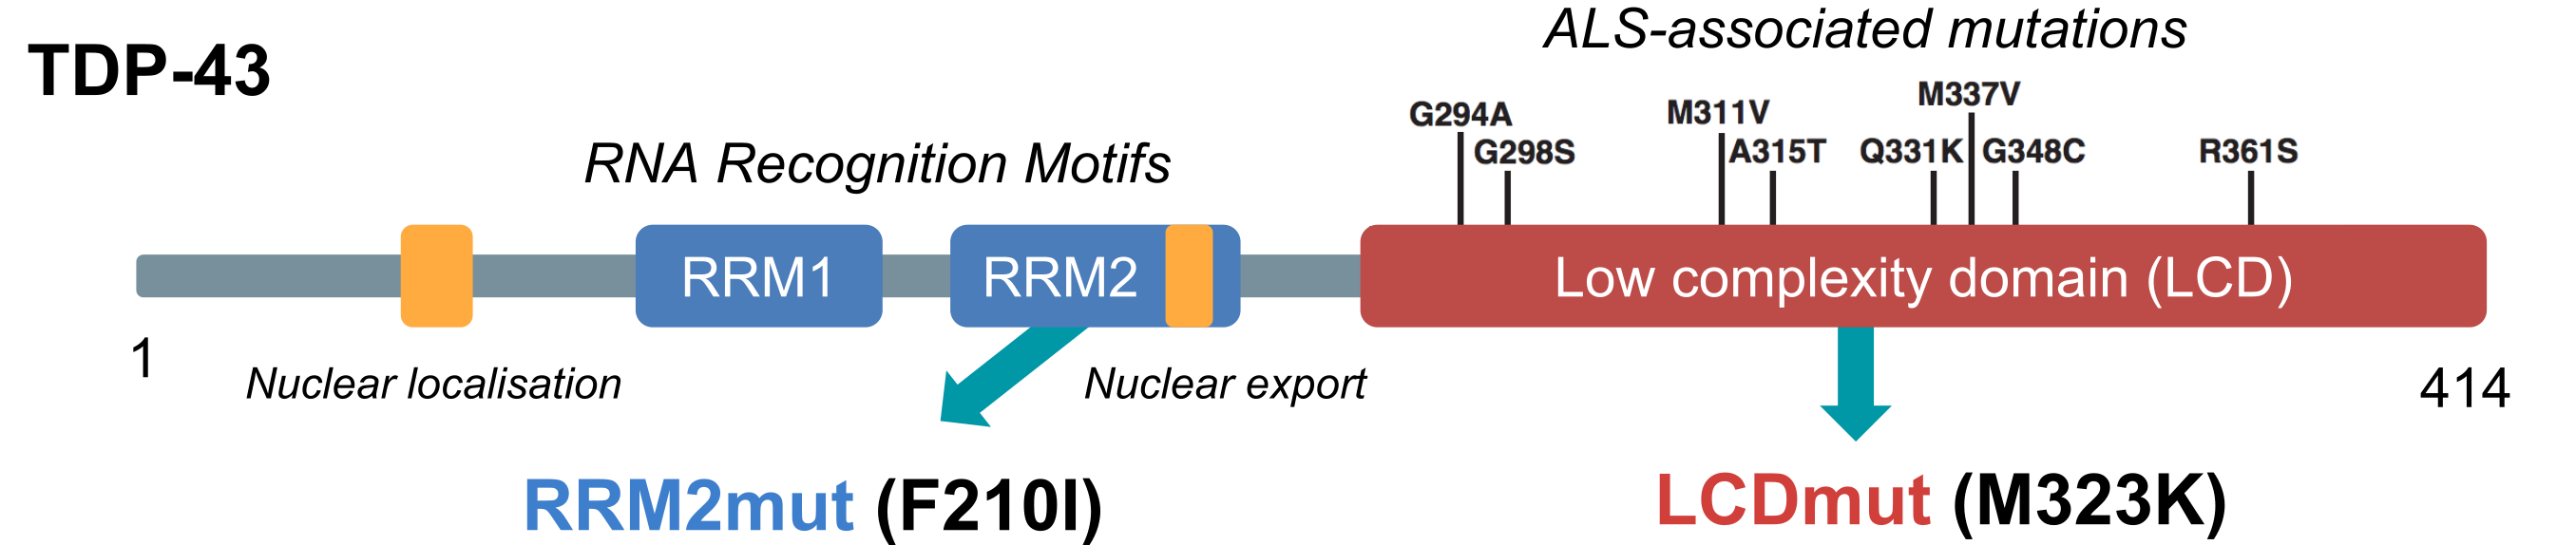
\includegraphics[width=\textwidth]{Figures/05_tdp_mice/TDP_structure_mutations.png}
	\caption[The two TARDBP mutations and their location within the TDP-43 protein]{
		\textbf{The two TARDBP mutations and their location within the TDP-43 protein.}
		RRM2mut affects the second RNA recognition motif whereas LCDmut affects the C-terminal low complexity domain.
	}
	\label{fig:tdp_structure}
\end{figure}

N-ethyl-N-nitrosourea (ENU) is a very potent mutagenic compound. Dosing male mice with ENU induces point mutations in sperm cells \citep{DeAngelis2000}. 
Large banks of mutant mouse sperm are maintained at MRC Harwell \citep{Acevedo2008} and the RIKEN in Japan \citep{Gondo2010}. 
From these resources two mouse lines with mutations in \textit{Tardbp} were chosen, F210I and M323K. 
The F210I mutation lies within the second RNA recognition motif (RRM2) of the TDP-43 protein whereas M323K lies within the C-terminal low complexity domain (LCD). 
This region is a hotspot for ALS mutations (Fig. \ref{fig:tdp_structure}). 
The M323K mutation lies within a 20 amino acid alpha-helical region previously found to be important for liquid phase separation and protein aggregation \citep{Conicella2016}. 
Developing these two mice allowed us to interrogate TDP-43 function and compare a mutation that would be predicted to impair the RNA binding ability of TDP-43 (F210I) with a mutation that potential resembles ALS (M323K). 
Due to their positions within the protein, the two mutations will be henceforth referred to as RRM2mut and LCDmut.

% info on breeding - F210I is embryonic lethal
We derived mice from mutant sperm and backcrossed for 10 generations onto a mixed C57BL/6J - DBA/2J background to remove unwanted background mutations.
RRM2mut is embryonic lethal in the homozygous state but not in heterozygosity, whereas homozygous LCDmut mice are viable and live normal lifespans. 
The two mutant lines were crossed together to create compound heterozygotes.
The RRM2mut/LCDmut mice were viable, suggesting the two mutations complement each other.
Close observation of aged LCDmut revealed gradual muscle weakness and a reduction in motor neuron numbers in the spinal cord (data not shown), suggesting that the patient-like M323K mutation indeed causes symptoms of neurodegeneration reminiscent of ALS. 
Due to the extreme differences in phenotype, particularly the neurodegeneration seen in LCDmut adults, I was curious to explore the effect of the mutations on RNA splicing.

\subsection{The two mutations have opposing effects on splicing known TDP-43 targets}

\begin{figure}[h!]
	\centering
	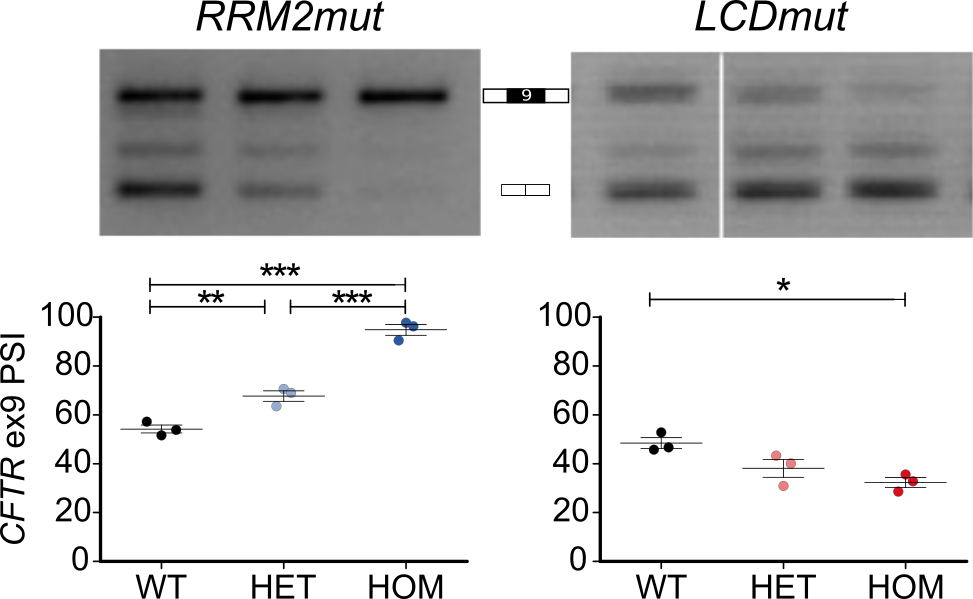
\includegraphics[width=10cm]{Figures/05_tdp_mice/CFTR.png}
	\caption[Opposite effects on splicing CFTR exon 9 minigene, a known TDP-43 splicing target]{
		\textbf{Opposite effects on splicing CFTR exon 9 minigene, a known TDP-43 splicing target.}
	RT-PCR traces from primers flanking CFTR exon 9, quantified as PSI ratios for each genotype. *** P < 0.0001 (ANOVA); ** P < 0.01; *** P < 0.001 (Tukey post-hoc test).
	}	
	\label{fig:CFTR}
\end{figure}

Exon 9 of the \textit{CFTR} gene was the first mRNA splicing target of TDP-43 to be described in the literature \citep{Buratti2001-et}. Knocking down TDP-43 leads to increased exon 9 inclusion, suggesting that TDP-43 acts to promote exon skipping. 
We made use of a minigene construct created from \textit{CFTR} exon 9 and its two flanking introns and exons \citep{Buratti2007minigene}.
Reverse-Transcriptase Polymerase Chain Reaction (RT-PCR) was performed to amplify between primers that flank exon 9. 
Analysis of the gel electrophoresis traces shows two primary bands: a larger band corresponding to exon 9 inclusion and a smaller band corresponding to exon 9 skipping. 
RRM2mut has a clear dose-dependent increase in exon 9 inclusion compared to skipping and thus resembles a loss of TDP-43 splicing function (Fig.  \ref{fig:CFTR}). 
Conversely, LCDmut has a dose-dependent increase in exon 9 skipping.
This suggests that the pro-skipping action of TDP-43 is increased at the CFTR locus and the LCDmut mutation causes a gain of splicing function.

%% INSERT TDP MEF SCATTERS
\begin{figure}[h]
	\centering
	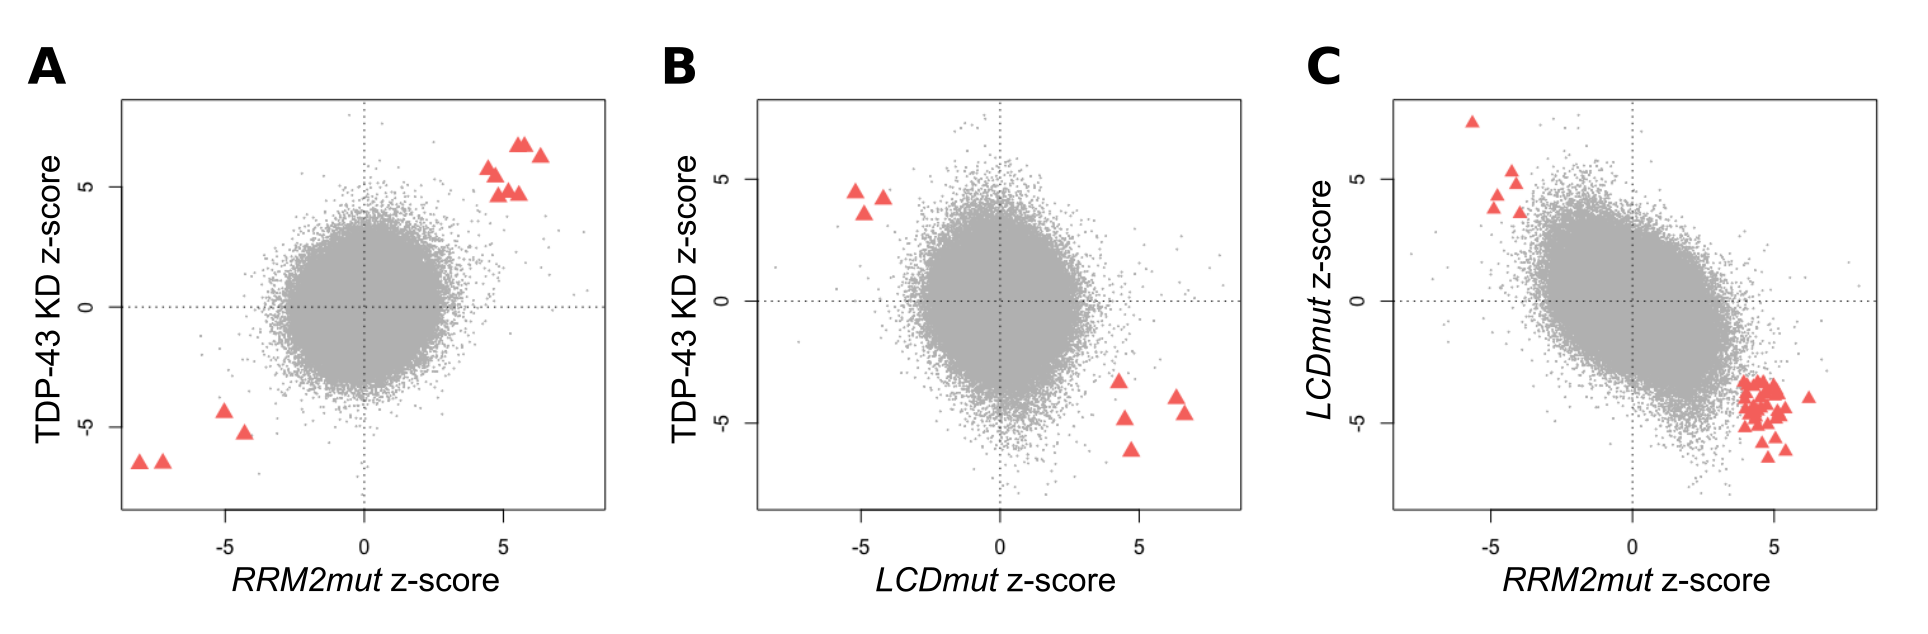
\includegraphics[width=\textwidth]{Figures/05_tdp_mice/mef_scatters.png}
	\caption[Comparing exon usage between the two mutations and a TDP-43 knockdown]{
		\textbf{Comparing exon usage between the two mutations and a TDP-43 knockdown.}
	Signed Z-scores for all exons found by DEXSeq in the mouse embryonic fibroblasts, comparing a TDP-43 shRNA knockdown to RRM2mut \textbf{(A)} and LCDmut \textbf{(B)} and comparing the two mutations \textbf{(C)}. Exons significant at FDR < 10\% plotted as red triangles, non-significant exons plotted as grey dots.
}
	\label{fig:mef_scatters}
\end{figure}

To look transcriptome-wide at the effects of the two mutations on simple cassette exon splicing the lab generated low-depth RNA-seq data from mouse embryonic fibroblasts. 
To compare both mutations to a simple loss of TDP-43 a short hairpin RNA (shRNA) was designed to be complementary to \textit{Tardbp} mRNA.
Binding of the shRNA should target \textit{Tardbp} mRNA for degradation, reducing TDP-43 protein levels. 
I performed a cassette exon splicing analysis and converted the fold change and \textit{P}-value from each exon into a signed Z-score. 
This allows for two way comparisons  between the shRNA knockdown of TDP-43 (TDP-KD), LCDmut and RRM2mut. 
Separating each graph into quadrants makes it clear that all significantly changed exons found in each mutation are changed in the same direction between RRM2mut and TDP-KD (Fig. \ref{fig:mef_scatters}). 
However, the exon changes are opposing when comparing LCDmut and TDP-KD, as well as between LCDmut and RRM2mut . 
This provides evidence at transcriptome scale that RRM2mut is a loss of splicing function whereas LCDmut is behaving oppositely.

%%CASSETTE EXON SCATTERS
\begin{figure}[h]
	\centering
	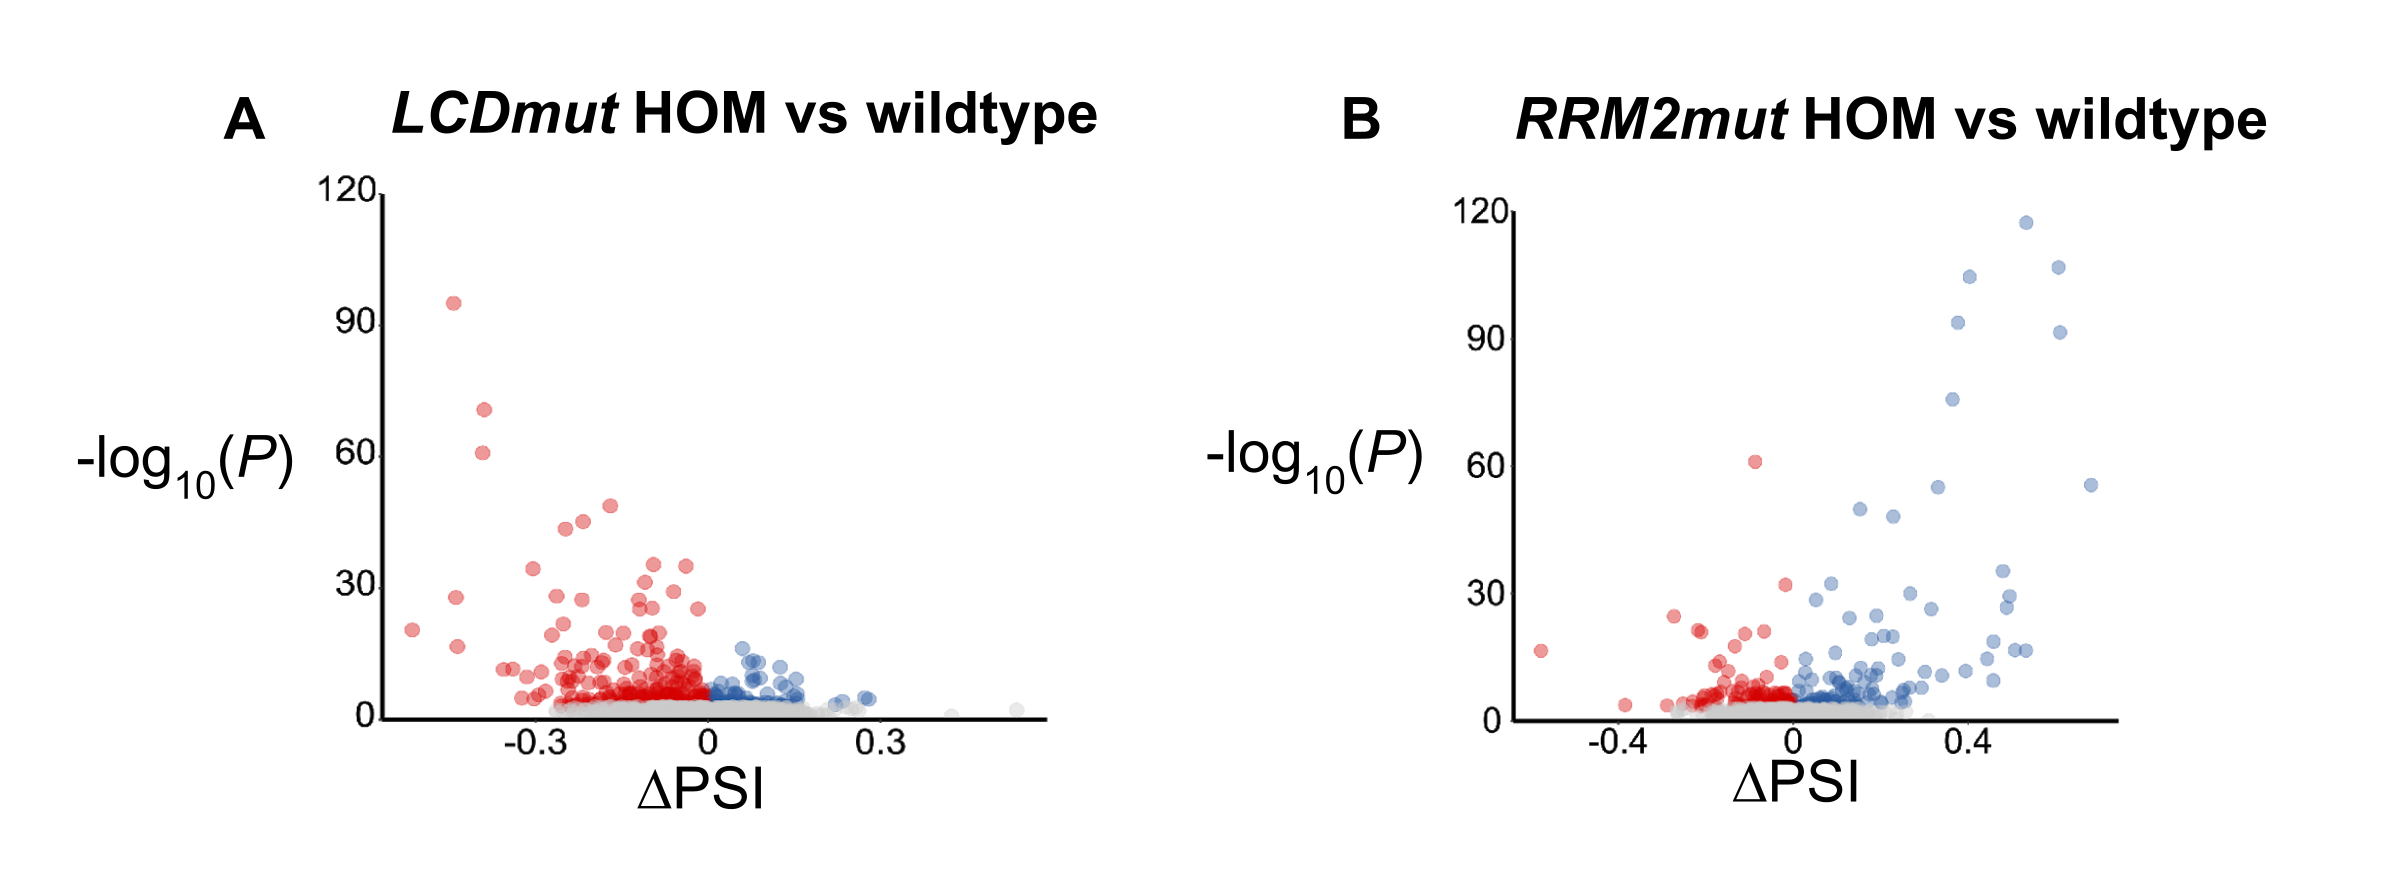
\includegraphics[width=\textwidth]{Figures/05_tdp_mice/transcriptome_scatters.png}
	\caption[Direction of cassette exon splicing in the two mutant lines]{
		\textbf{Direction of cassette exon splicing in the two mutant lines.}
	All splicing events found by SGSeq plotted by \textit{P}-value and direction ($\Delta$PSI; see methods) for LCDmut \textbf{(A)} and RRM2mut \textbf{(B)}.
}
	\label{fig:cassette_scatters}
\end{figure}

To deeply interrogate splicing changes at time points that were relevant to the phenotypes of interest (death in RRM2mut and neurodegeneration in LCDmut) high depth RNA-seq data was generated from RRM2mut embryonic brains and LCDmut adult brains (30 days post-natal). 
Higher depth and longer read data allows for better discrimination of novel splicing events and so I ran a novel splicing analysis using SGSeq \citep{Goldstein2016}. 
Plotting the direction and \textit{P}-value of all cassette exons found in the two mutations strongly suggests that the strongest splicing changes are in exon inclusion in RRM2mut and in exon skipping in LCDmut (Fig. \ref{fig:cassette_scatters}).

% RNAmaps of the cassettes - motif and iCLIP
\begin{figure}[h]
	\centering
	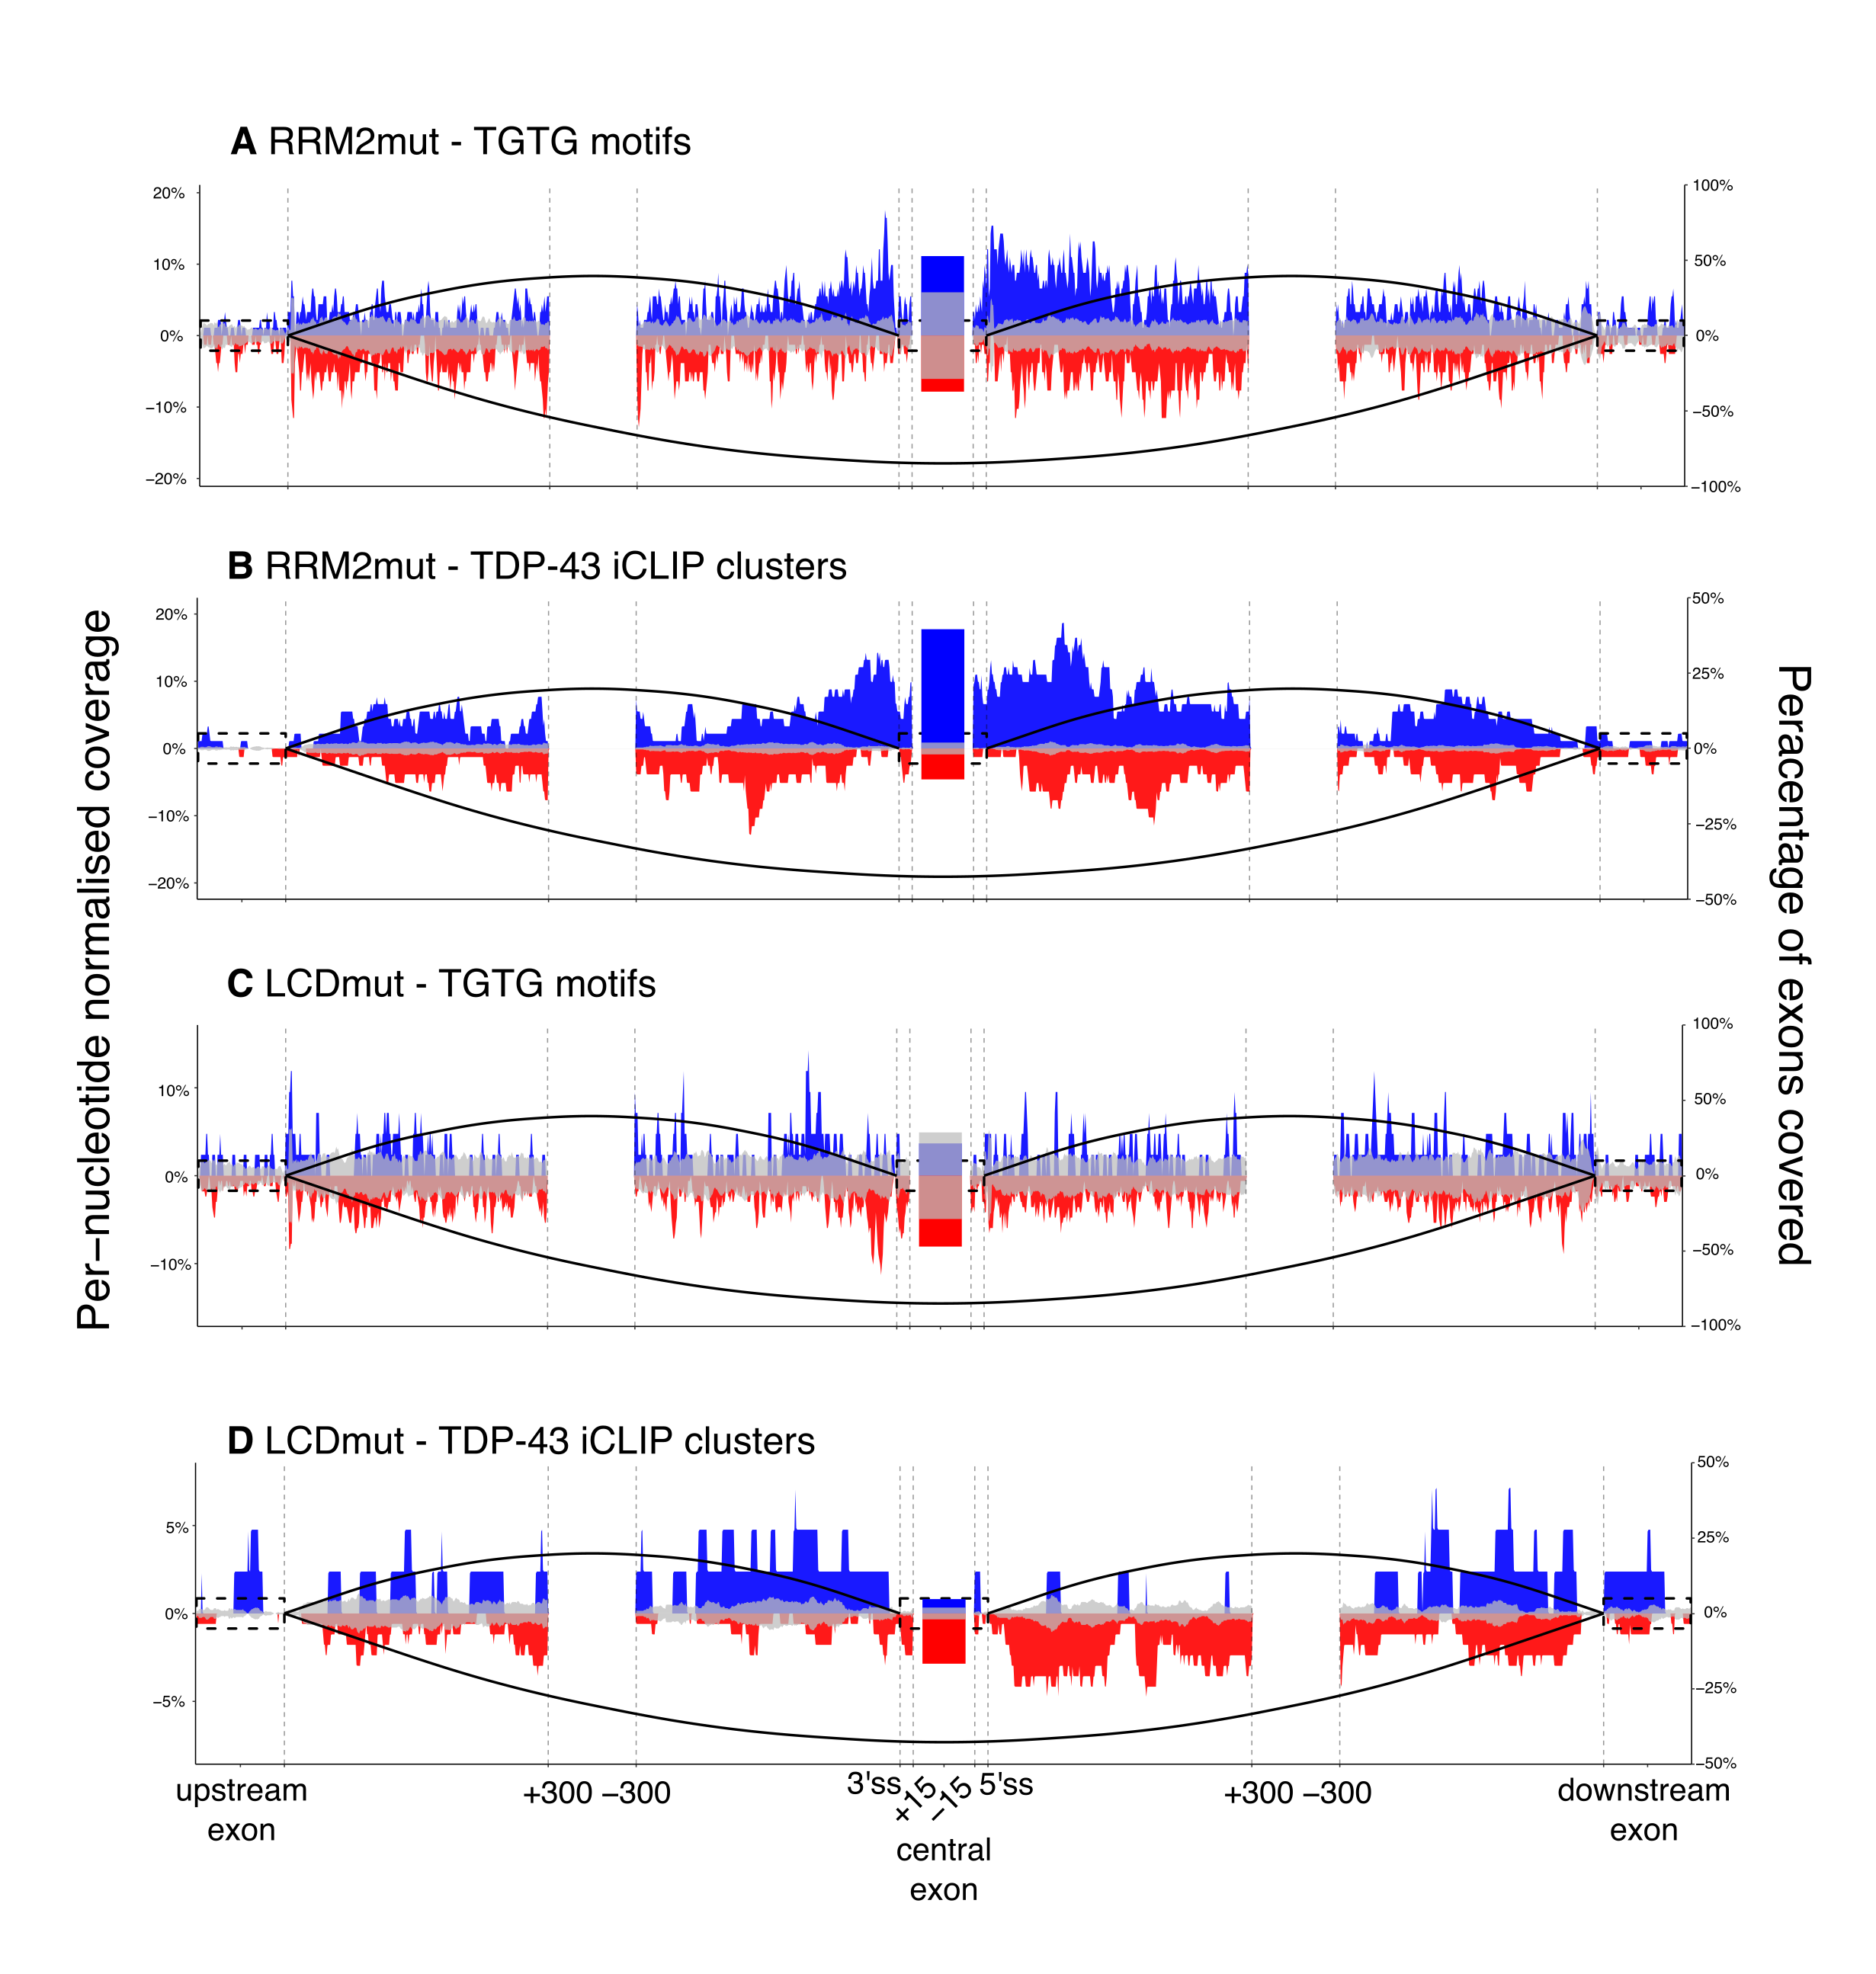
\includegraphics[width=14cm]{Figures/05_tdp_mice/RNAmap_cassettes.png}
	\caption[RNA maps visualise positional enrichment of iCLIP and sequence motifs]{
		\textbf{RNA maps visualise positional enrichment of iCLIP and sequence motifs within cassette exon splicing loci.}
	RNA maps constructed from differentially included (blue) and skipped (red) cassette exons.  
	\textbf{(A)} TGTG motifs in RRM2mut.
	\textbf{(B)} TDP-43 iCLIP in RRM2mut.
	\textbf{(C)} TGTG motifs in LCDmut; 
	\textbf{(D)} TDP-43 iCLIP in RRM2mut.
	}
	\label{fig:RNAmap_cassettes}
\end{figure}

The splice-site competition model of cassette exon splicing allow an RNA-binding protein to either repress or enhance cassette exon splicing depending on the position it binds within the intron. When RNA binding proteins bind on top of or close to an exon, the recognition of that exon's splice sites by the spliceosome is blocked and the exon is no longer included in a transcript. Conversely, if an RNA binding protein binds deeper within the intron it can act to recruit the spliceosome to the exon and enhance exon inclusion. 
% CITATIONS - PTBP, NOVA etc
I created RNA maps to look for positional enrichment within and around the the cassette exons, both for UGUG sequence motifs as well as RNA-protein interaction information from iCLIP experiments. For each set of exons I used a random set of 1994 cassette exons which were not significantly changed as a null distritbution.
Motif-based maps were calibrated using the invariant AG and GT dinucleotides at the 3' and 5' splice sites respectively (see appendices).
For RRM2mut, the 91 cassette exons with increased inclusion were enriched in UGUG sequence motifs (Fig \ref{fig:RNAmap_cassettes}A) and iCLIP peaks (Fig \ref{fig:RNAmap_cassettes}B).
Both sequence features either directly overlap the exon or are within 100 bp either side. 
The 78 skipped exons  in RRM2mut were depleted in both feature types directly on top and close by. 
LCDmut cassette exons show the inverse distribution to RRM2mut as the 168 skipped exons are enriched for features that directly overlap and closely flank the exons (Fig \ref{fig:RNAmap_cassettes}C/D), whereas the 42 included exons were depleted of sequence features that were close or overlapping.
All exons howed enrichment of TDP-43 features at the distal flanking 5' and 3' splice sites, suggesting long range cooperation around the distal splice sites.
This data suggests that whereas the RRM2mut cassette exons are shifted due to a reduction in TDP-43, the LCDmut exons are shifting in a direction suggesting an increase of TDP-43 in the mutant cells.

% include numbers!
%RNAmaps
%RRM2mut casssette exons: included 91, skipped 78, control 1994
%LCDmut cassette exons:  42, 168, 1994


\subsection{RRM2mut leads to a loss of splicing function and cryptic exons}

%% CRYPTIC EXONS IN RRM2mut
\begin{figure}[h!]
	\centering
	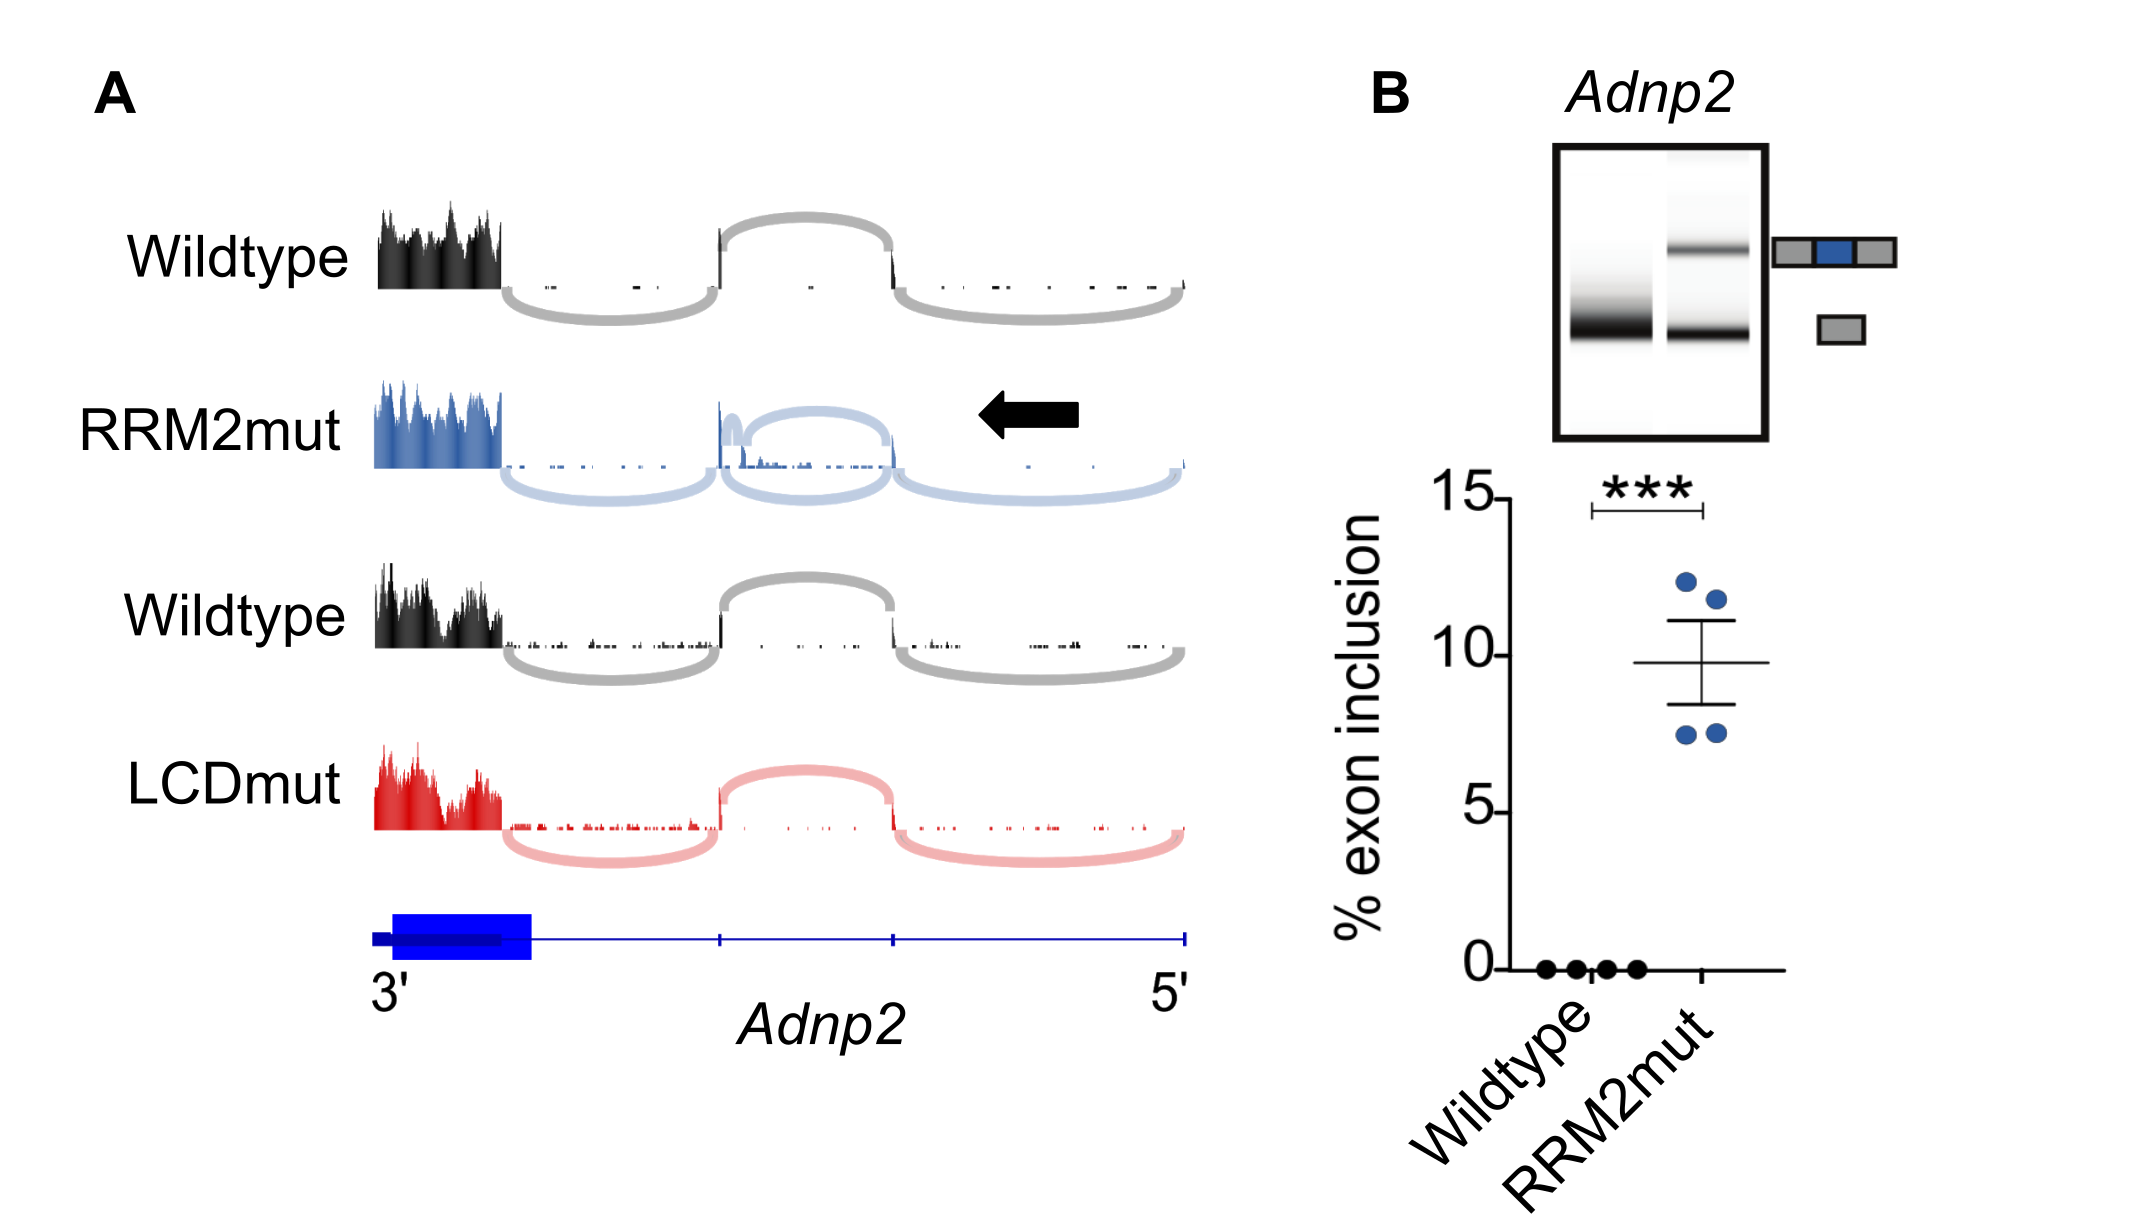
\includegraphics[width=14cm]{Figures/05_tdp_mice/cryptic_exon_multi.png}
	\caption[RRM2mut leads to cryptic exon splicing]{
		\textbf{RRM2mut leads to cryptic exon splicing.}
	\label{cryptic_multi}
	\textbf{(A)} Representative RNA-seq traces show cryptic exon in \textit{Adnp2} included in RRM2mut specifically. 
	\textbf{(B)} RT-PCR of \textit{Adnp2} selectively amplifies a band corresponding to cryptic exon inclusion in RRM2mut samples. P < 0.001; t-test(two-sided).
}
\end{figure}

A hallmark of TDP-43 depletion is the widespread inclusion of non-conserved cryptic exons \citep{Ling2015}. The bias towards cassette exon inclusion suggested that a number of RRM2mut repressed exons may be cryptic exons. Rather than relying on isoform annotation I filtered all cassette exons found in RRM2mut and selected those that were barely or not at all spliced in wildtypes but were included in RRM2mut samples, resulting in 33 candidate cryptic exons being discovered. A representative example of a cryptic exon in \textit{Adnp2} is shown in Fig. \ref{cryptic_multi}, changing from 0\% inclusion in wildtype mice to ~10\% inclusion in RRM2mut but not in LCDmut mice.  

%% LONG GENES 
\begin{figure}[h]
	\centering
	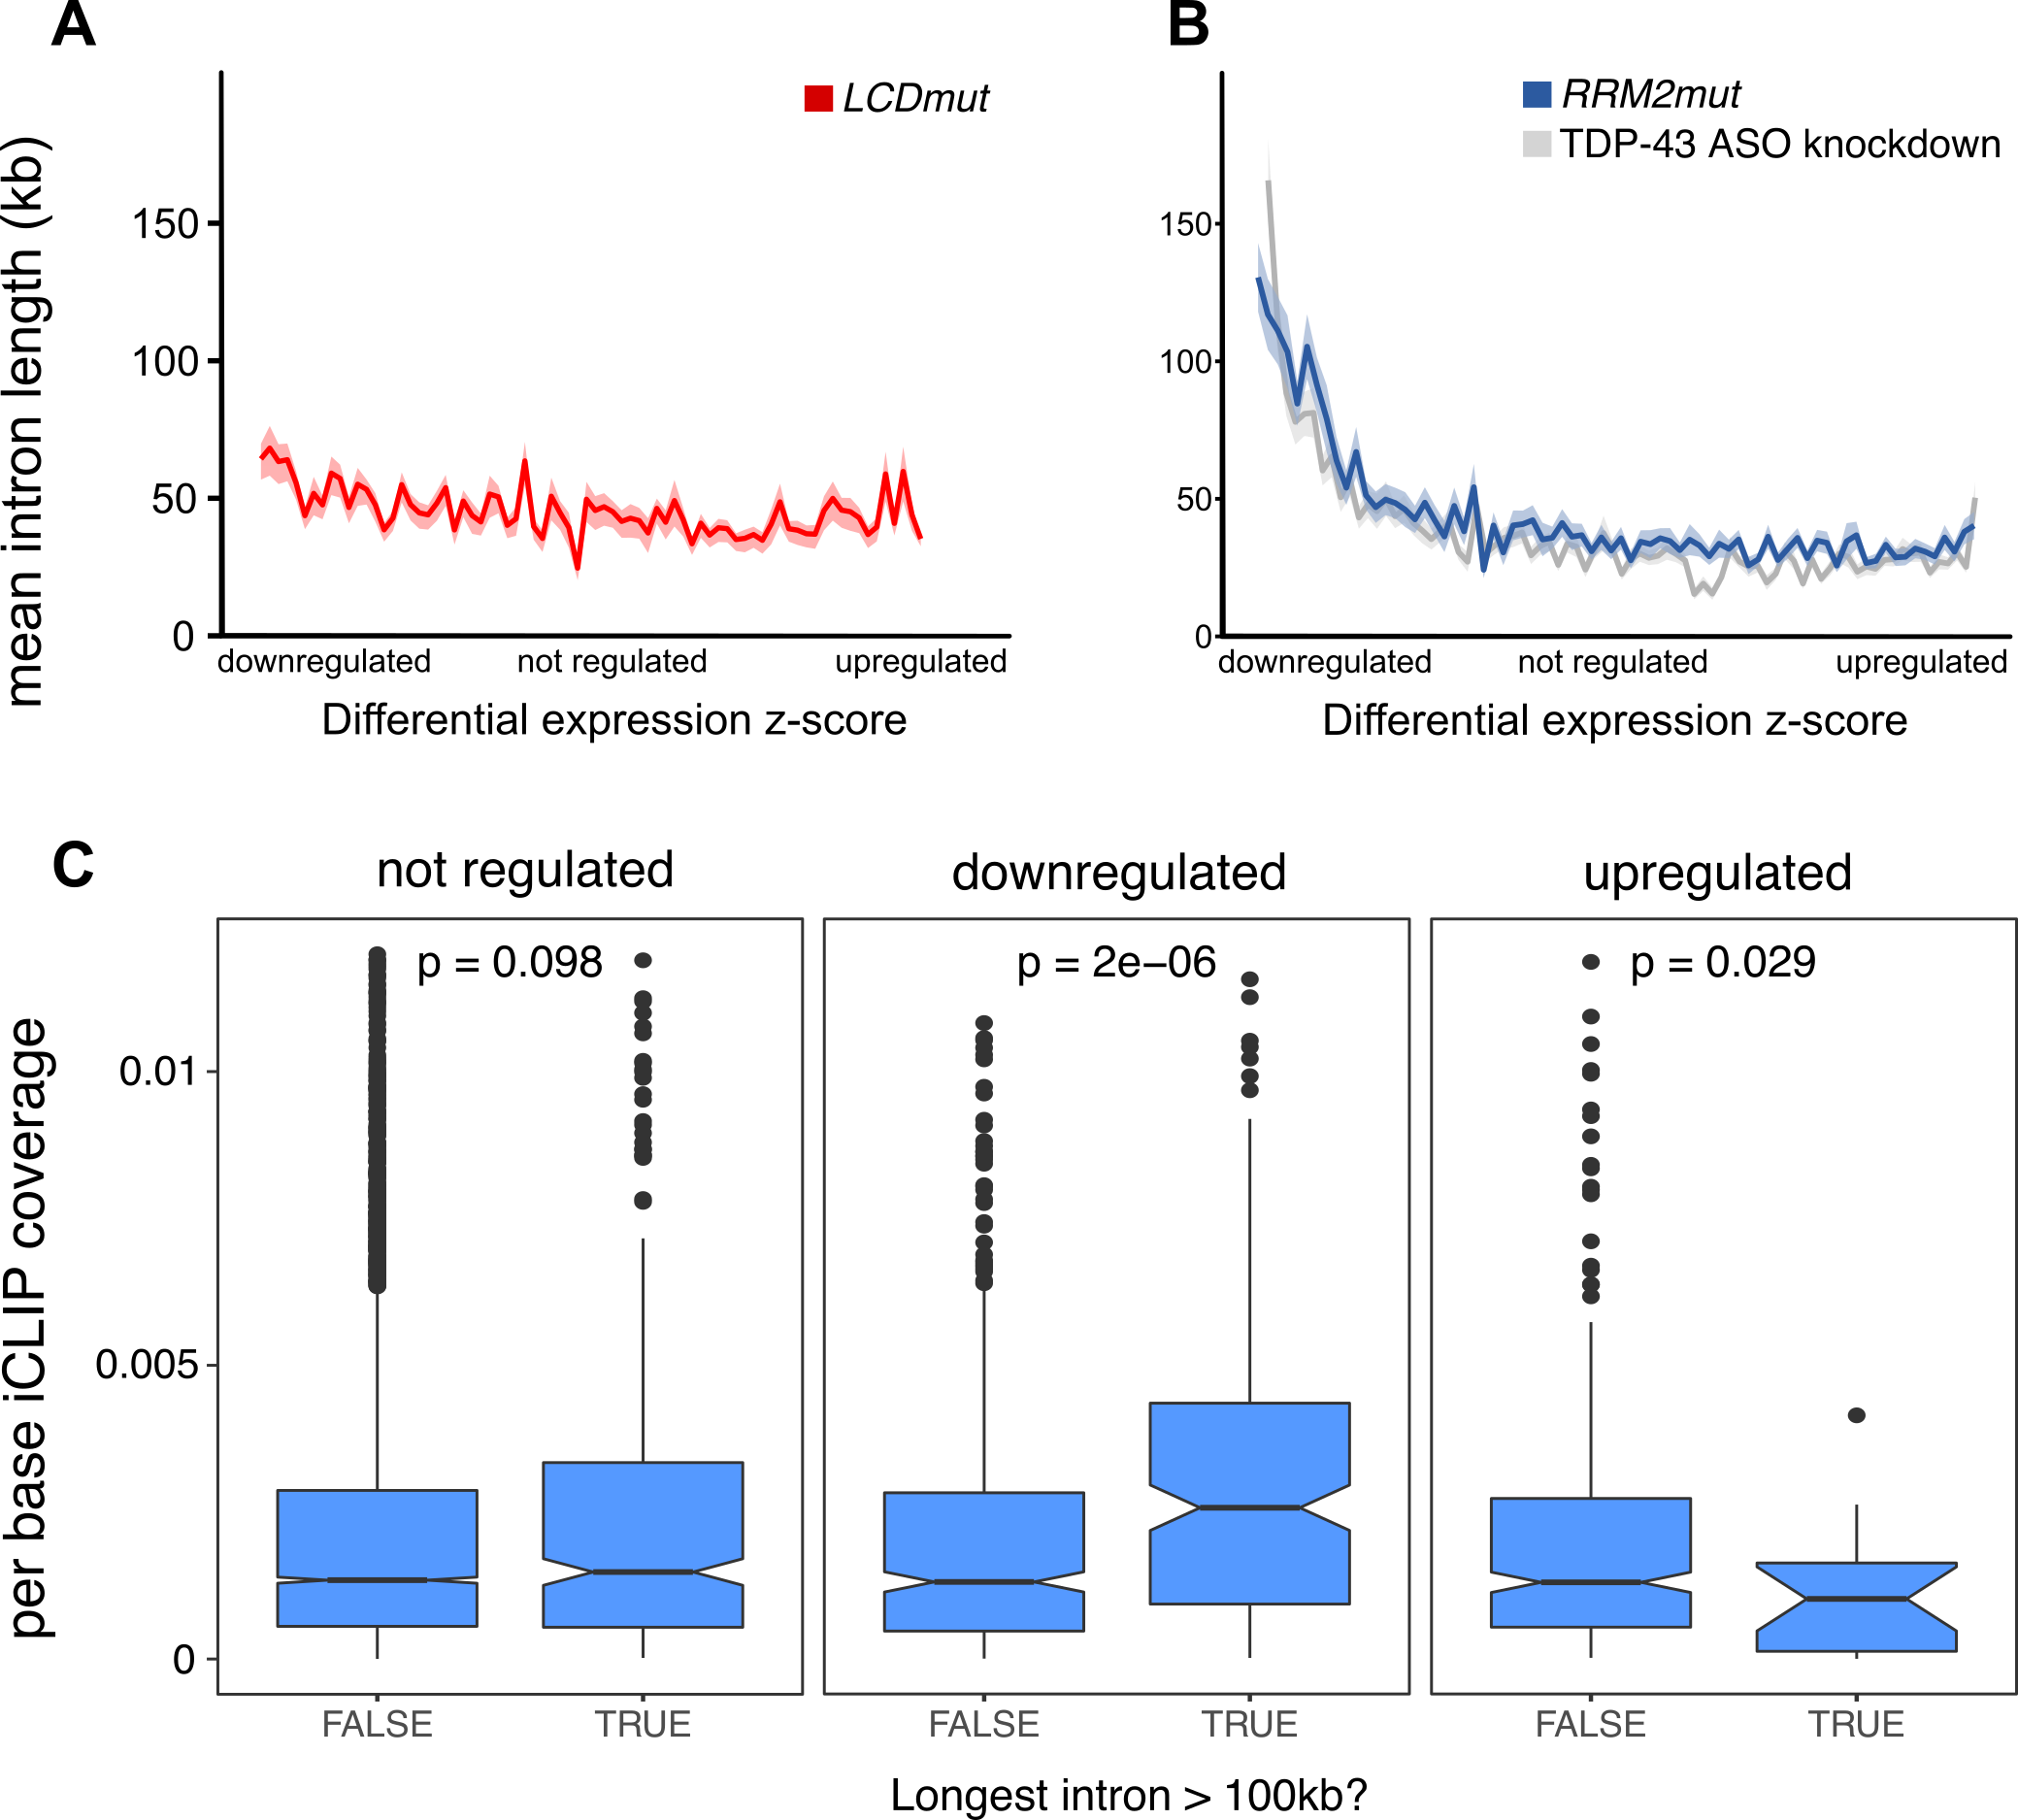
\includegraphics[width=12cm]{Figures/05_tdp_mice/long_genes_multi.png}
	\caption[RRM2mut gene expression has bias for long gene downregulation]{
		\textbf{RRM2mut gene expression has bias for long gene downregulation, mirroring TDP-43 knockdown data.}
	\textbf{(A,B)} Mean intron length in kilobases for bins of genes ordered by signed Z-score. TDP-43 antisense olignucleotide (ASO) knockdown data taken from \cite{Polymenidou2011-hs}. \textbf{(C)} The per-nucleotide overlap of iCLIP interaction peaks for each gene is significantly increased in long intron genes downregulated in RRM2mut mice compared to wildtype. \textit{P}-values are from Mann-Whitney-Wilcoxon test.
}
	\label{fig:long_genes}
\end{figure}

Another feature of TDP-43 loss of function is a striking downregulation of genes with long introns (>100kb). This phenomenon was first observed in mice where an antisense oligonucleotide strategy was used to lower TDP-43 in the striatum (TDP-ASO); \citep{Polymenidou2011-hs}. Long intron genes are over-represented in neuronal cells \citep{Sibley2015} and it is thought that TDP-43 binds within these long introns to promote their processing and splicing. I re-analysed RNA-seq data from this study and compared it to the RRM2mut and LCDmut sequencing data. I ran a differential gene expression analysis with DESeq2 and ranked all genes by their direction of expression change between controls and ASO treatment/mutations. I then binned genes into groups of 200 and extracted the lengths of longest intron in each gene from GENCODE annotation. While in LCDmut, gene length is evenly distributed between downregulated, unchanged and upregulated genes (Fig. \ref{fig:long_genes}A), there is a clear bias for the most downregulated genes having long introns in both RRM2mut and TDP-ASO (Fig. \ref{fig:long_genes}B). An orthogonal approach is to look at TDP-43 protein-RNA interaction data performed on wildtype cells with the iCLIP method \citep{Huppertz2014-ip}. I calculated the proportion of nucleotides in each gene that had an iCLIP peak overlapping, suggesting direct TDP-43 binding. Genes that were downregulated in RRM2mut had no difference in the distribution of iCLIP peak overlaps except for those downregulated genes that also contained at least one intron longer than 100 kilobases (\textit{P}=2e-6; Fig. \ref{fig:long_genes}C). Long intron genes were modestly depleted in iCLIP peaks when the genes were upregulated (\textit{P}=0.029).


\subsection{LCDmut shows the inverse of cryptic splicing - skiptic splicing}

\begin{figure}[h!]
	\centering
	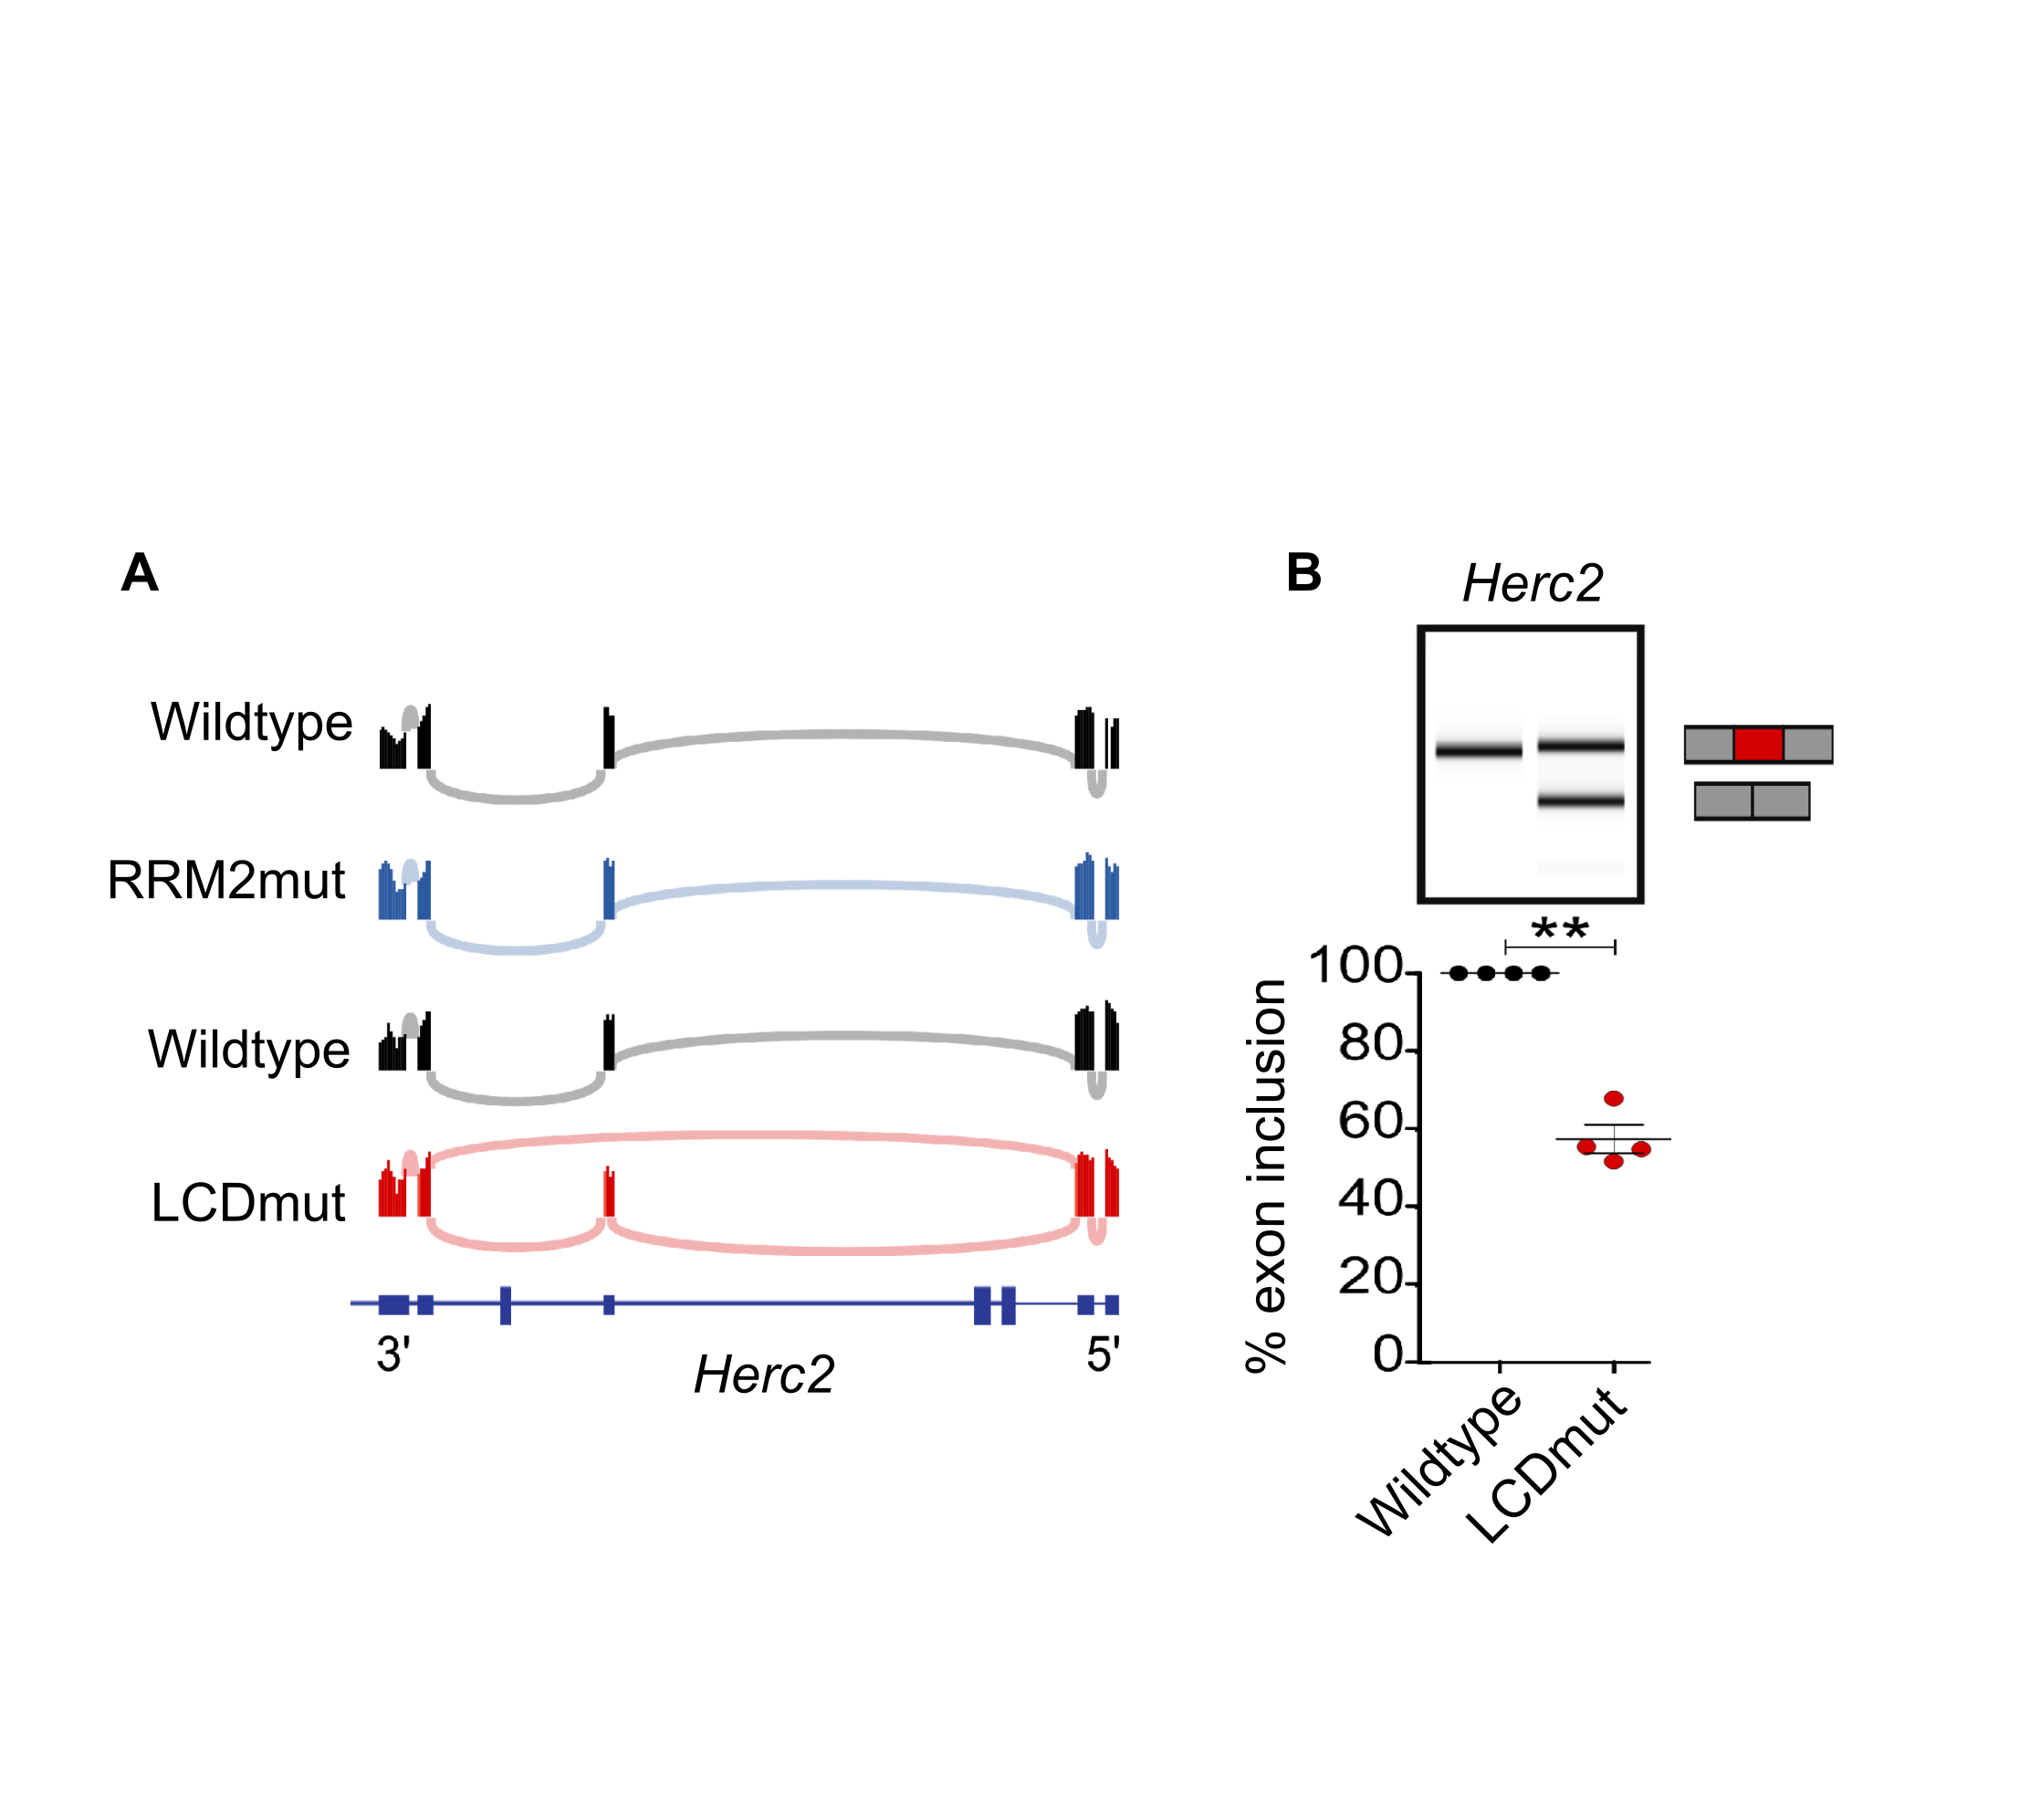
\includegraphics[width=12cm]{Figures/05_tdp_mice/skiptic_exon_multi.png}
	\caption[LCDmut leads to skiptic exon splicing]{
		\textbf{LCDmut leads to skiptic exon splicing.}
	\textbf{(A)} Representative RNA-seq traces show a constitutive exon in \textit{Herc2} skipped in LCDmut specifically - a skiptic exon. 
	\textbf{(B)} RT-PCR of \textit{Herc2} selectively amplifies a band corresponding to exon skipping skipping in LCDmut samples. P < 0.001; t-test(two-sided). 
	\textbf{(C)} PhyloP conservation scores for 1000 randomly chosen mouse exons compared to the 48 skiptic exons found in LCDmut.
}
	\label{fig:skiptic_multi}
\end{figure}

I applied the same cryptic exon filtering strategy to LCDmut and found a small number of potential cryptic exons. However, when applying the inverse critera to find exons that are 95-100\% included in wildtype and then skipped in LCDmut I uncovered 48 exons. These exons are constitutively spliced in wildtype samples and yet are skipped in LCDmut, making them the inverse of cryptic exons. I therefore christened them "skiptic" exons - a portmanteau of cryptic and skipping. A selection of skiptic exons were validated by RT-PCR (Fig. \ref{fig:skiptic_multi}). 


\begin{figure}[h!]
	\centering
	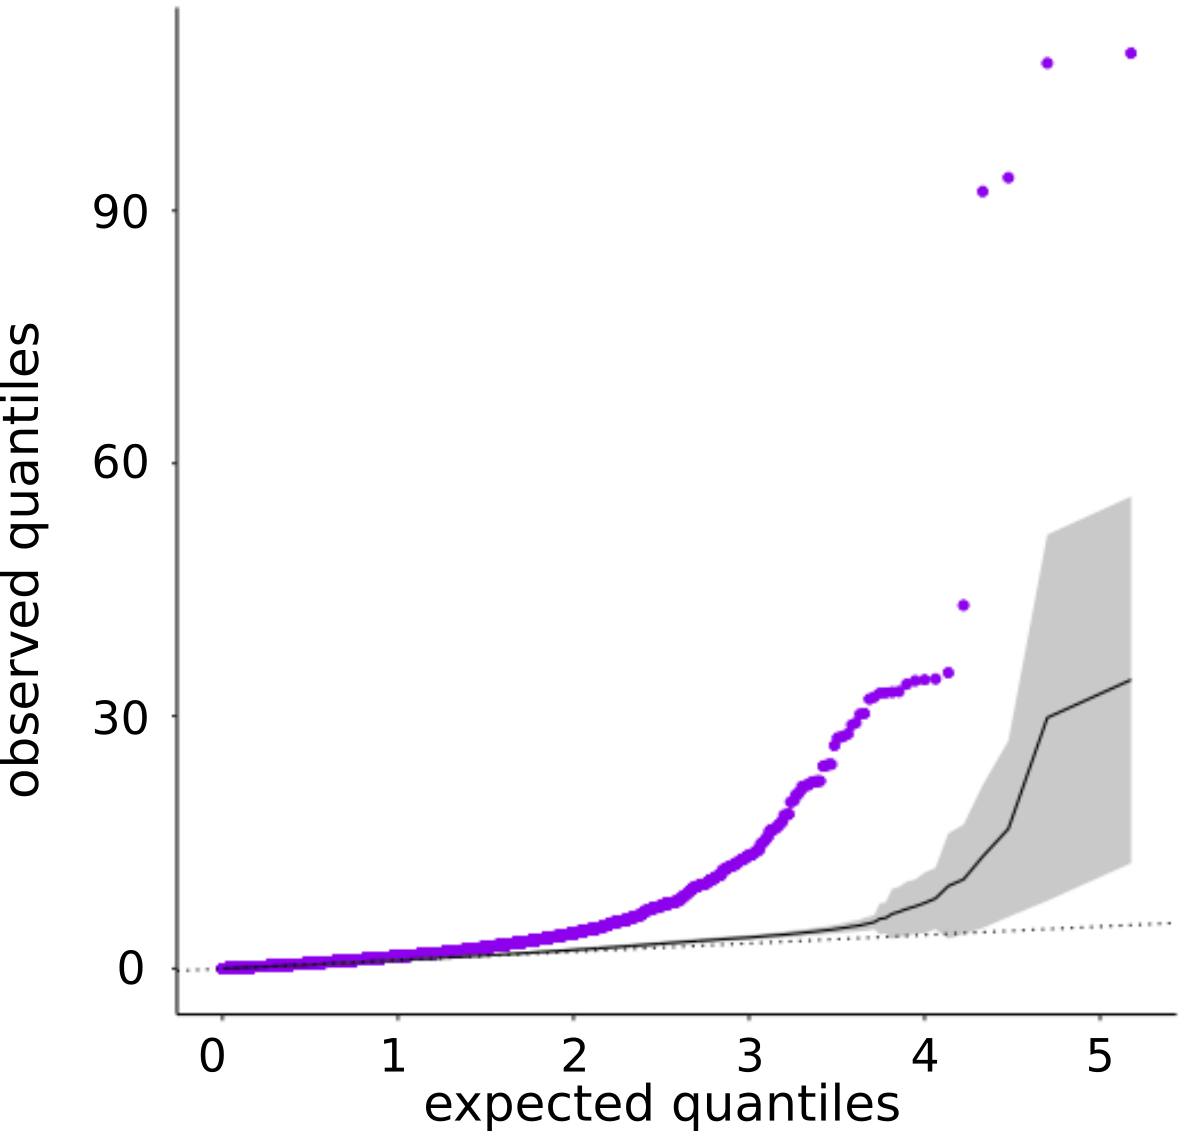
\includegraphics[width=7cm]{Figures/05_tdp_mice/permutation_ribbon.png}
	\caption[Permuting sample order shows clear splicing difference between LCDmut mice and controls]{
		\textbf{Permuting sample order shows clear splicing difference between LCDmut mice and controls.}
		Quantile-quantile plots show the difference between expected and observed distribution of \textit{P}-values generated from multiple tests. True case-control sample labelling of LCDmut and littermate controls (purple) shows clear inflation of low \textit{P}-values when compared to all permutations of sample ordering (grey; plotted as mean $\pm$ standard deviation).
	}
	\label{fig:permutation}
\end{figure}

To demonstrate that the 48 skiptic exons found in LCDmut were not statistical anomalies due to the small sample size I employed a permutation strategy.
 The wildtype and LCDmut labels were shuffled 50 times to cover all possible sample orders and the splicing analysis repeated with the permuted labels. 
A quantile-quantile plot contrasts the observed distribution of \textit{P}-values generated by a large number of statistical tests with the theoretical expected distribution. 
If there is no difference between genotypes then some low \textit{P}-values are expected by chance due to the small sample size and the large number of tests. 
However, there is a clear difference in splicing between LCDmut and wildtype mice that drives a large inflation in the number of low \textit{P}-value splicing events far away from the expected distribution (Fig. \ref{fig:permutation}).
A table of counts of all exons found at each permutation is presented in the appendices.   


\subsection{Both skiptic and cryptic splicing show evidence of direct TDP-43 binding}

\begin{figure}[h!]
	\centering
	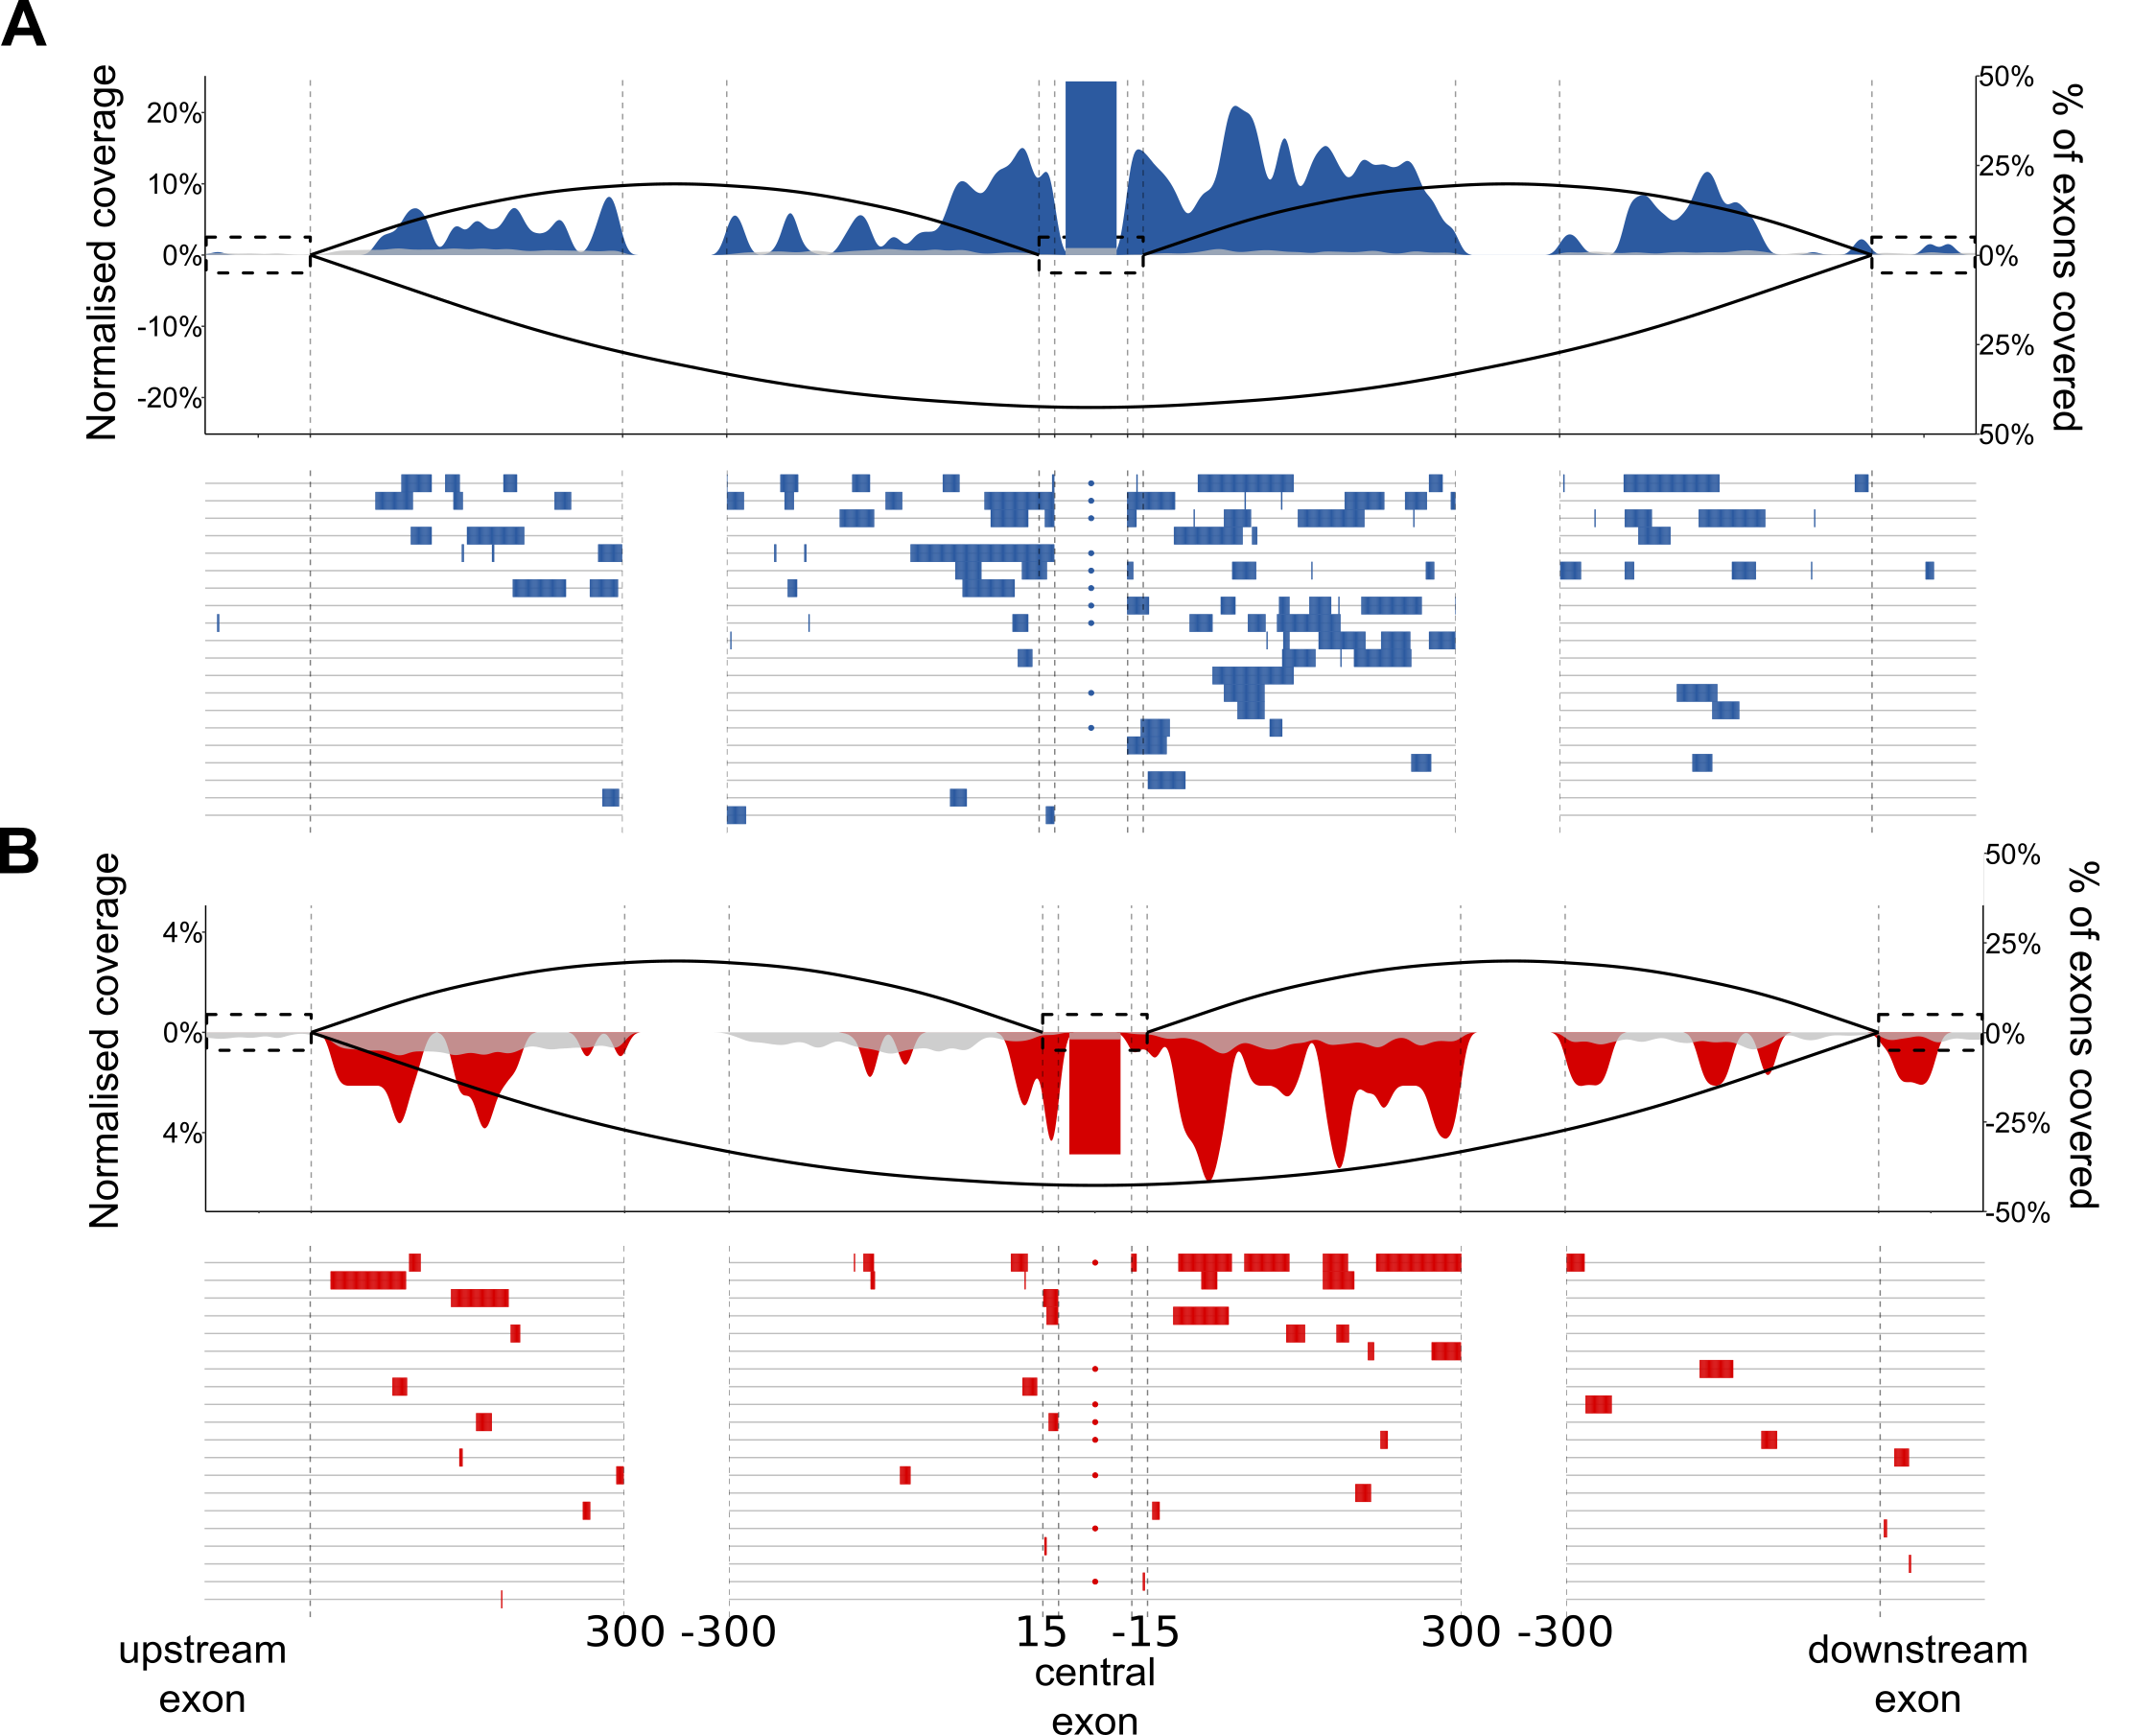
\includegraphics[width=\textwidth]{Figures/05_tdp_mice/iclip_multipanel.png}
	\caption[RNA maps of skiptic and cryptic exons show direct binding by TDP-43]{
		\textbf{RNA maps of skiptic and cryptic exons show direct binding by TDP-43.}
	\textbf{(A)} The 33 cryptic exons found in the RRM2mut embryonic mice. Traces show normalised iCLIP peak coverage within and around each exon. Left y-axis: the proportion of exons with an iCLIP peak at that nucleotide. Right y axis: the proportion of central exons or flanking exons that overlap any iCLIP peaks. Below, individual positions of iCLIP peaks for the top 20 cryptic exons. Circles in the centre denote whether there are any iCLIP peaks overlapping the central exon. 
	\textbf{(B)} as before for the 48 skiptic exons found in the LCDmut adult mice.
}
	\label{iclip_multi}
\end{figure}

Cryptic exons associated with TDP-43 depletion have been demonstrated to originate from mRNA that is directly bound by TDP-43 itself \citep{Ling2015}. 
This suggests that these splicing changes emerge because TDP-43 can no longer act to repress cryptic exon recognition by the splicing machinery and other factors. 
I remade the RNA maps for iCLIP protein-RNA interaction peaks for the 33 cryptic and 48 skiptic exons found in RRM2mut and LCDmut to test whether they appeared to be directly bound by TDP-43. 
The RRM2mut cryptic exons show overlapping and closely flanking TDP-43 binding and strikingly so do the LCDmut cryptic exons. 
Importantly, the iCLIP data used for these maps is mainly drawn from wildtype TDP-43, suggesting that while TDP-43 may be normally binding the skiptic exons it does not do so sufficiently strongly to repress their inclusion. 

\begin{table}
	\begin{footnotesize}
	\begin{tabular}{llll}
		& total & overlap	& \% \\
		\hline
		All exons in GENCODE vM12 &	744,786	& 37,276 & 5\% \\
		All constitutive exons found in all samples	& 239,897	& 17,828	& 7.4\% \\
		All cassette exons found in all samples &	5,656 &	361	& 6.4\% \\
		Significant cassette exons (FDR < 0.05) between LCDmut and wildtype mice	& 260	& 49 & 18.8\% \\
		Skiptic exons (control PSI > = 0.95; dPSI > = -0.05; FDR < 0.05) & 47 &	31 & 66\% \\
	\end{tabular}
	\end{footnotesize}
	\caption[Proportions of exons with any TDP-43 binding from iCLIP]{\textbf{Proportions of exons with any TDP-43 binding from iCLIP}}
	\label{tab:iclip_proportions}
\end{table}


\subsection{Skiptic splicing is predicted to be deleterious to gene expression}

\begin{figure}[h!]
	\centering
	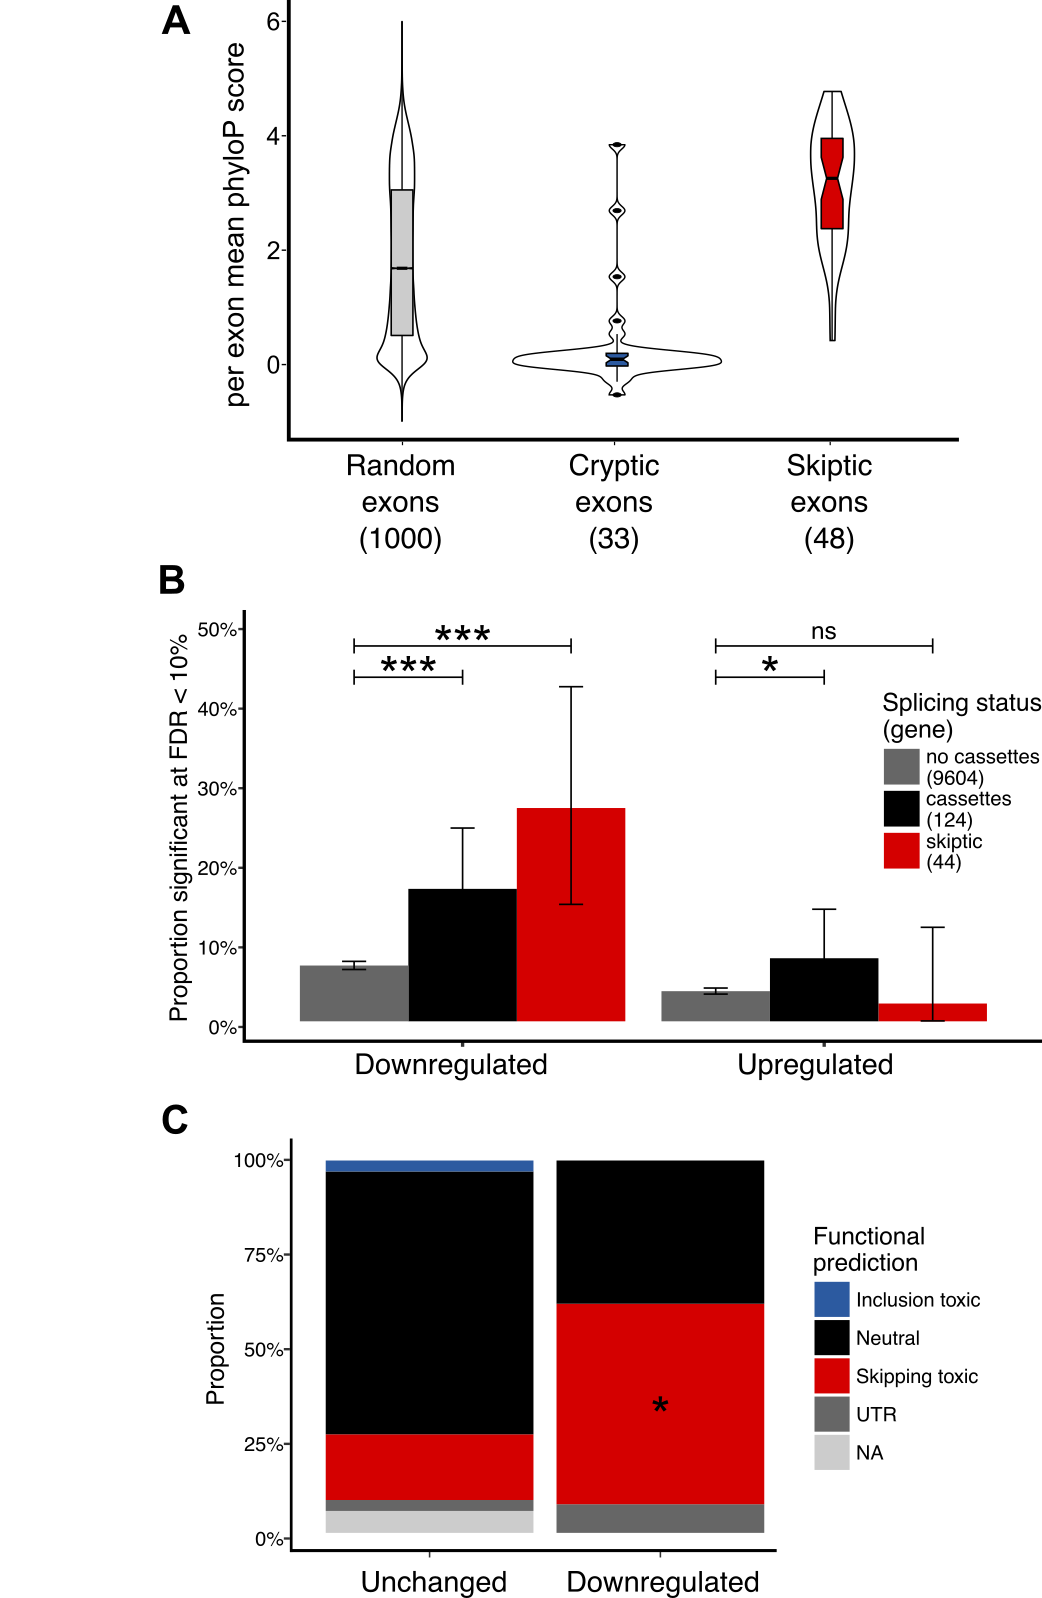
\includegraphics[width=9cm]{Figures/05_tdp_mice/functional_plots_vertical.png}
	\caption[Functional analyses of the skiptic exons]{
		\textbf{Functional analyses of the skiptic exons.}
	\textbf{(A)} Per-exon mean PhyloP conservation scores presented as box plots for each set of exon, showing the median and interquartile range. Notches are the 95\% confidence interval of the median. 
	\textbf{(B)} The relationship between splicing status and differential expression in LCDmut. Significantly downregulated genes (FDR < 0.1) are enriched in skiptic exons compared to genes expressed at a similar level (\textit{P}=1.19e-6), as well as non-skiptic cassette exons (\textit{P}=6.16e-5). Upregulated genes are mildly enriched in non-skiptic cassette exons (\textbf{P}=0.029) but not in skiptic exons (\textbf{P}=0.88). All \textit{P}-values generated from a binomial test. 
	\textbf{(C)} Proportions of predicted downstream consequence of exon skipping for either non-regulated or downregulated skiptic exons. \textit{P}=0.034; chi-squared test.
}
	\label{fig:functional_plots}
\end{figure}

Cryptic exons originate from very poorly conserved DNA sequence  (Fig. \ref{fig:functional_plots}A), suggesting that there is no functional protein coding information encoded in them. 
Inclusion of these essentially randomised sequences would more likely than not lead to degradation of the host mRNA transcript through the inclusion of premature stop codons or frameshifts and nonsense-mediated decay.
Skiptic exons are highly conserved (Fig. \ref{fig:functional_plots}A), with a much higher average conservation level than a randomly chosen set of annotated exons from GENCODE.  
This is to be expected from their close to 100\% inclusion rates within transcripts. 
Their constitutive splicing status means that their inclusion is near guaranteed and so unlike cassette exons, which are swapped in and out dynamically between tissues and developmental time points, I hypothesis that there is no evolutionary pressure to maintain a length divisible by 3. 
In the event of these exons being skipped they would likely lead to a shift of reading frame, potentially leading to degradation of the host transcript through nonsense-mediated decay.
 To test whether skiptic exon splicing correlated with host transcript degradation I combined the differential splicing and differential expression analyses together. I separated genes into sets based on i) whether they were significantly upregulated or downregulated in LCDmut compared to wildtype (FDR < 10\%) and ii) whether they contained either a cassette exon or a skiptic exon that changed in inclusion levels between LCDmut and wildtype (FDR < 1\%). 
 Genes that contained skiptic exons were more likely to be downregulated than those without any cassette exon splicing  (\textit{P}=1.19e-6; binomial test; Fig. \ref{fig:functional_plots}B). The same trend cannot be seen in the other direction as there as no increased likelihood for skiptic containing genes to be upregulated. 
 Finally I attempted to predict \textit{in silico} whether the skipping of a skiptic exon would lead to nonsense mediated decay. 
 By combinining the central cassette exon with the flanking upstream exons and translating the concatenated sequence it is possible to assess whether skipping the central exon would frameshift the downstream exon, generating premature stop codons. 
 Using this method I discovered that 15 out of 47 of the skiptic exons would lead to the inclusion of a premature stop codon.  
I compared the distribution of predictions between skiptic exons in downregulated and unchanged genes and found an increased representation of predictions of toxic skipping from 18\% to 54\% (\textit{P}=0.034; chi-squared test). 

\subsection{LCDmut impairs TDP-43 autoregulation}

\begin{figure}[h!]
	\centering
	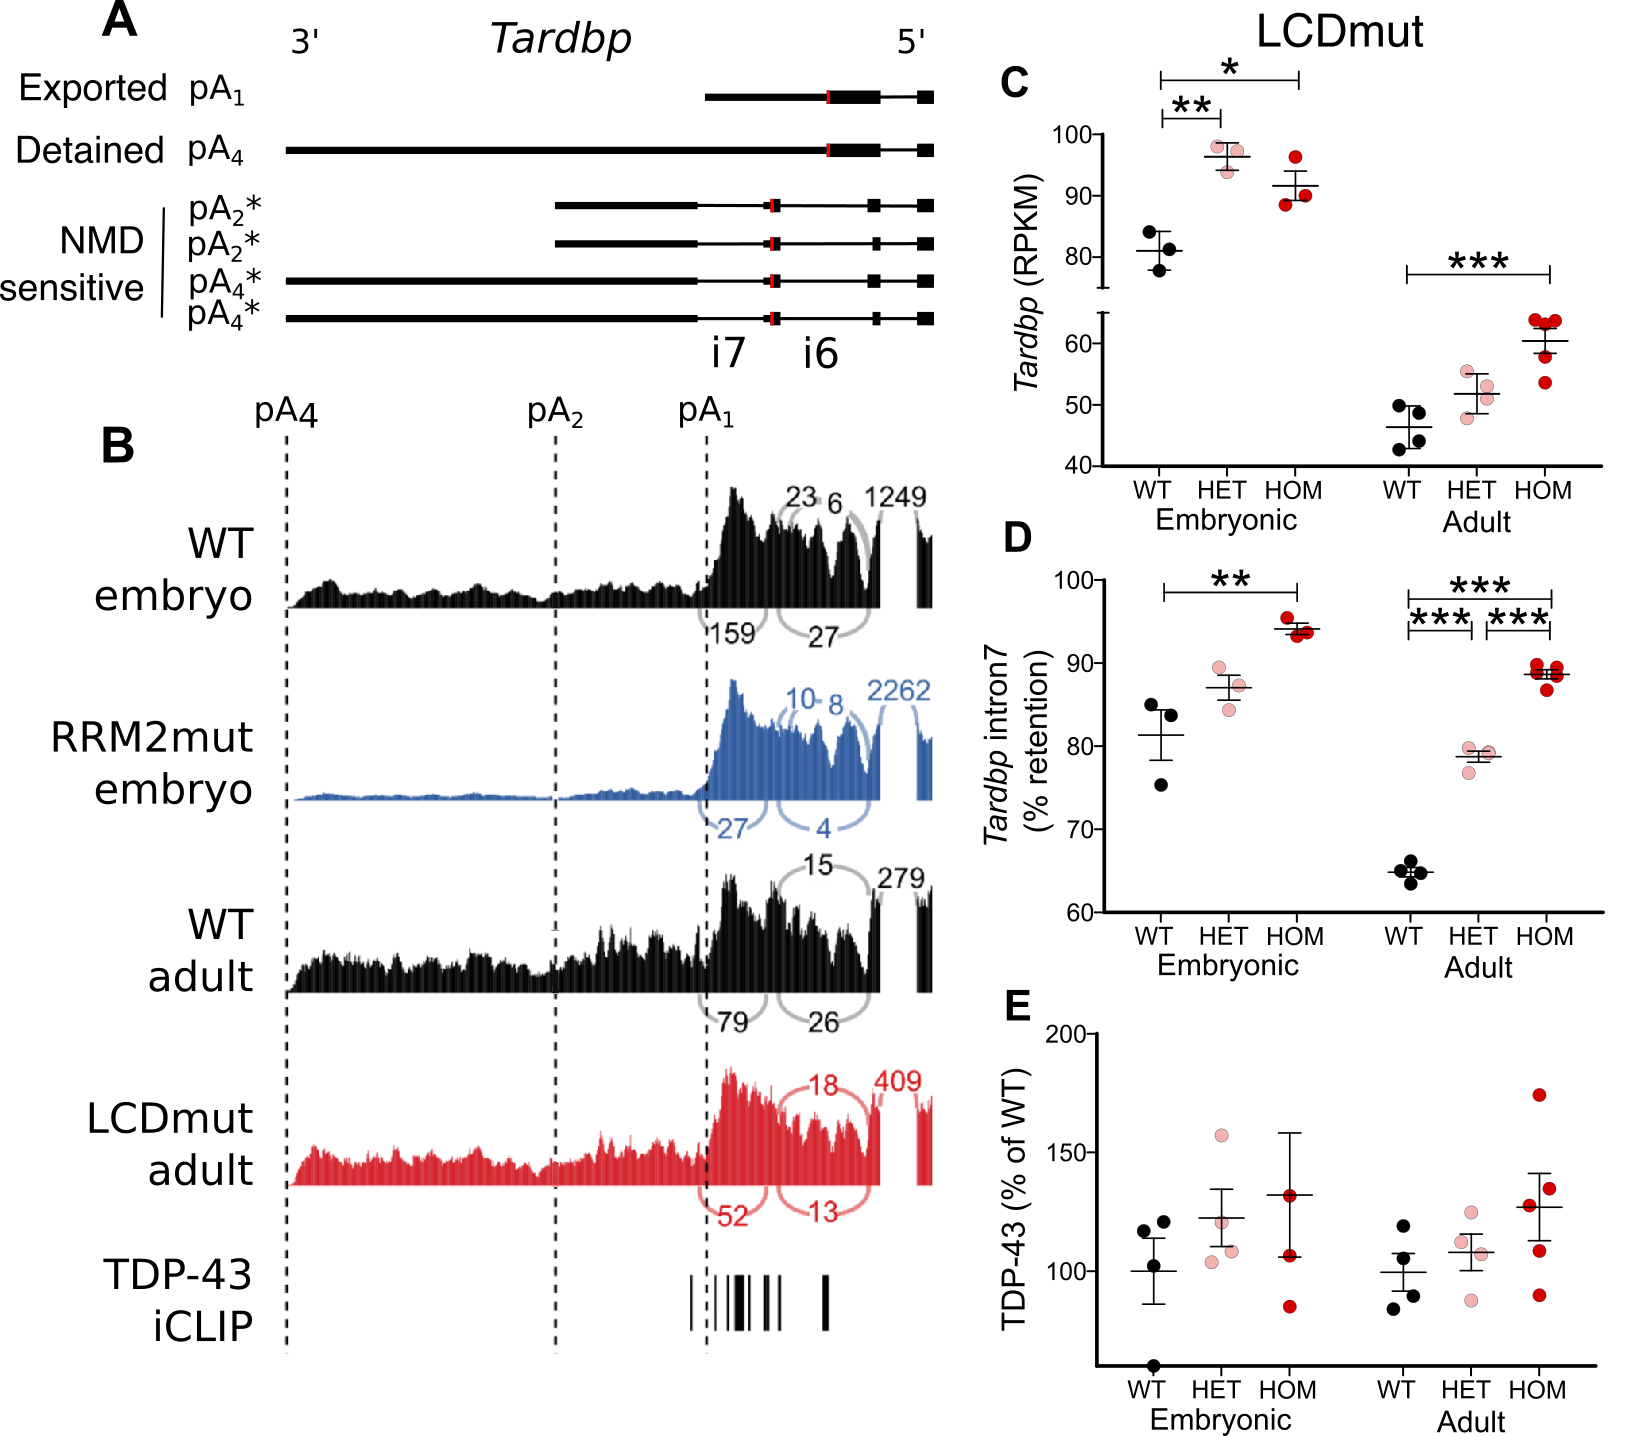
\includegraphics[width=\textwidth]{Figures/05_tdp_mice/autoregulation.png}
	\caption[LCDmut and TDP-43 autoregulation]{
		\textbf{LCDmut and TDP-43 autoregulation.}
	\textbf{(A)} The 3'UTR of \textit{Tardbp}. At least six potential 3'UTR isoforms have been proposed by \citep{Koyama2016}, consisting of 3 different polyadenylation (pA) sites. * indicates that this isoform is predicted to be degraded by nonsense-mediated decay. Stop codons indicated by red bars. 
	\textbf{(B)} Expression of all \textit{Tardbp} isoforms (RPKM) increases in LCDmut at two time points.  Embryonic dataset ANOVA, \textit{P}=0.0032, \textit{n}=3; adult dataset ANOVA, \textit{P}=0.0009, \textit{n}=4$-$5; error bars: SD; Bonferroni multiple comparison tests are plotted as \textit{P}-value: *\textit{P} < 0.05; **\textit{P} < 0.01; ***\textit{P} < 0.001
	\textbf{(C)} Retention of 3'UTR intron 7 increases in LCDmut. Embryonic dataset ANOVA, \textit{P}=0.0113, \textit{n}=3; adult dataset ANOVA, \textit{P} < 0.0001, \textit{n} = 4$-$5; error bars: SEM; Bonferroni multiple comparison tests are plotted as \textit{P}-value: **\textit{P} < 0.01; ***\textit{P} < 0.001.
	\textbf{(D)} Quantification of TDP-43 protein levels in relation to $\beta$-actin in Western blots. Results are normalised to the mean of wildtype (100\%). Embryonic dataset: ANOVA \textit{P}=0.480, \textit{n}=4; adult dataset: ANOVA \textit{P}=0.491, \textit{n}=3; error bars: SD.
}
	\label{fig:autoregulation}
\end{figure}

Many RNA-binding proteins have been shown to regulate their own translation, this is termed autoregulation \citep{Lareau2007,Wollerton2004}]. 
When levels of the protein are high they will bind to their mRNA and shift production to an untranslated isoform, through nonsense-mediated decay or through nuclear retention \citep{McGlincy2008-wh,Boutz2015}.
The 3' untranslated region (3'UTR) of \textit{Tardbp} is remarkably complex regulatory hub (Fig. \ref{fig:autoregulation}A). 
There are 3 experimentally validated polyadenylation and cleavage sites, pA1, 2, and 4. 
There also 2 introns within the 3'UTR (6 and 7; \citep{Ayala2011,Koyama2016}). 
3'UTR splicing is a mechanism for regulating TDP-43 translation as an intron that follows a stop codon should trigger nonsense-mediated decay. 
Both spliced isoforms pA$_2$* and pA$_4$* are predicted to undergo nonsense-mediated decay due to the stop codon is further than 50bp from the intron in each.
Additionally, the long pA4 site is preferentially retained in the nucleus where it is degraded by the exosomal complex \citep{Ayala2011}.
Only the pA1 isoform is translated into TARDBP protein \citep{Koyama2016}.
TDP-43 binds the 3'UTR of its own mRNA overlapping the pA$_1$ site  \citep{Polymenidou2011,Tollervey2011}.
This prevents polyadenylation at the pA1 site and encourages the creation of the retained pA4 transcript and the splicing of NMD-sensitive pA$_2$* and pA$_4$* isoforms \citep{Koyama2016}. 
This system allows TDP-43 protein levels to regulate the stabilty of \textit{Tardbp} mRNA.

I assessed the the \textit{Tardbp} 3'UTR locus in the RNA-seq data to observe whether the two mutations had effects on autoregulation. 
RRM2mut shifts the balance of UTR isoforms from near equal amounts of pA$_1$ and pA$_4$ to predominantly pA$_1$, presumably due to its reduced RNA binding ability  (Fig. \ref{fig:autoregulation}A).  
In LCDmut, a clear upregulation of Tardbp mRNA expression is seen in both embryonic and adult RNA-seq samples (Fig. \ref{fig:autoregulation}B). 
When I quantified the level of intron 7 inclusion,  a proxy for the proportion of NMD-sensitive pA$_2$* and pA$_4$* isoforms, LCDmut increased intron 7 retention in a dose dependent manner, suggesting a loss of NMD-sensitive UTR isoforms (Fig. \ref{fig:autoregulation}C). 
However, when assessing the total TDP-43 protein levels by Western blotting, no difference was observed between LCDmut and wildtype cells (Fig. \ref{fig:autoregulation}D).
Together this suggests a subtle impairment in the autoregulation feedback loop in LCDmut cells.

\subsection{Skiptic splicing can be observed in human ALS patients}
% work performed by Pras - show RT-PCRs
% explain dodgy quantification
\begin{figure}[h!]
	\centering
	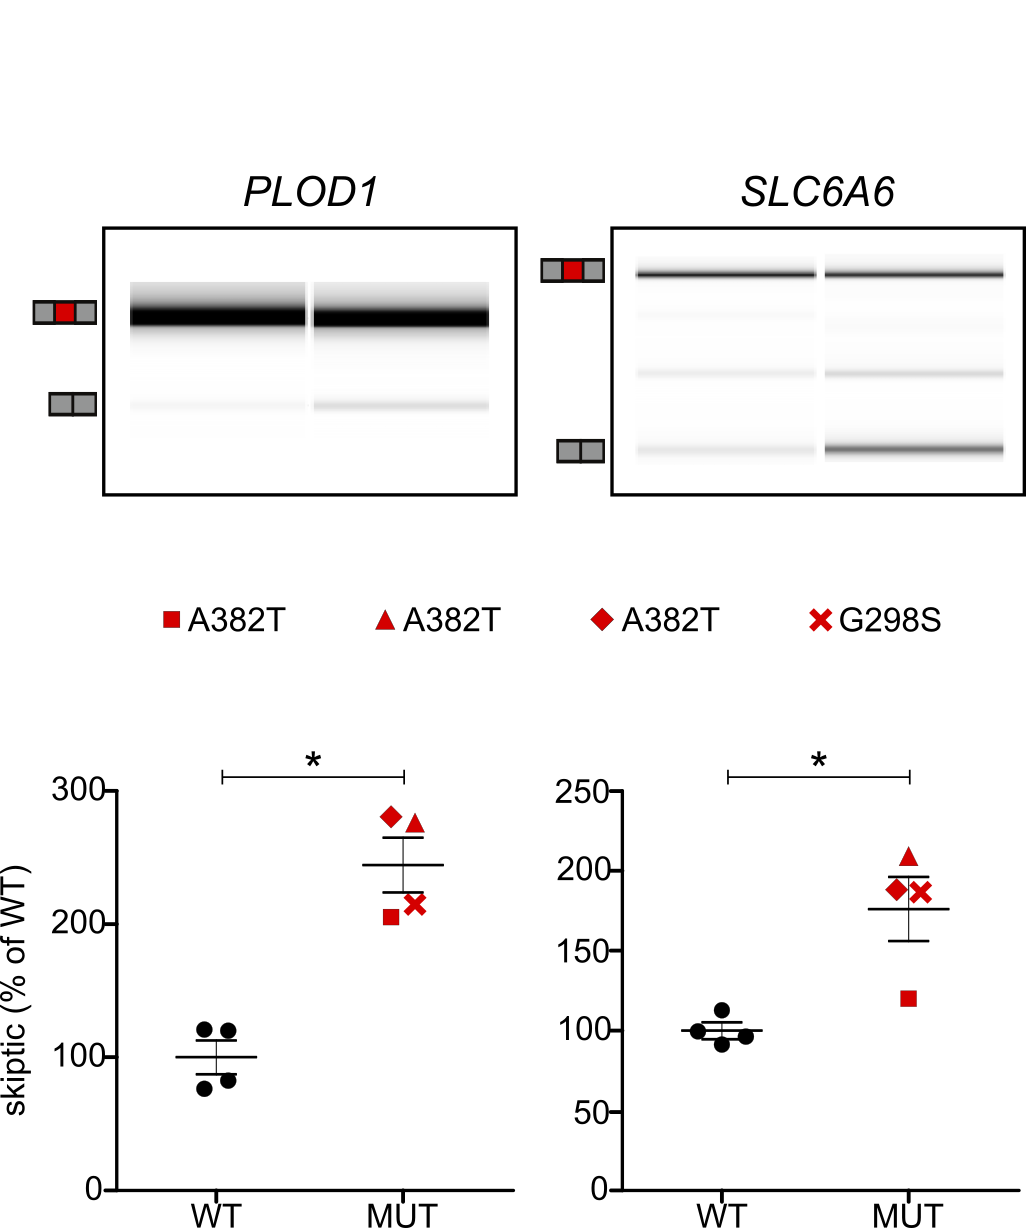
\includegraphics[width=10cm]{Figures/05_tdp_mice/skiptic_patients.png}
	\caption[Skiptic exon splicing in TARDBP ALS]{
		\textbf{Skiptic exon splicing in TARDBP ALS.}
		RT-PCR traces for two skiptic exons in fibroblasts taken from 4 \textit{TARDBP} ALS patients and 4 non-neurological control lines. For clarity, quantification was taken of the skiptic exon band only instead of the ratio. *\textit{P} < 0.05, \textit{n} = 4, error bars: SEM
	}
	\label{fig:skiptic_patients}
\end{figure}

Due to the high species conservation of the skiptic exons, I reasoned that it might be possible to see evidence of their skipping in human ALS patients with heterozygous mutations in the low complexity region of \textit{TARDBP}. Seven skiptic exons were tested using RT-PCR in four patients with the A382T and G298S mutations and four control fibroblast lines. 
Two skiptic exons were found to have a mild but statistically signficant increase in the intensity of the band matching the skipping transcript.	
This provides the first evidence of a gain of TDP-43 splicing function in patients with ALS-associated \textit{TARDBP} mutations.

\clearpage

\section{Discussion}

In this study  two complementary mouse models were developed to study the splicing function of TDP-43. 
%Benefits of knock-in mutations
%RRM2mut is softer LOF - allows mice to live longer and us to study embryonic tissues - role in development? Cite Modic paper
By using point mutations I have been able to observe the modulation of TDP-43-regulated splicing without dramatically altering TDP-43 expression. 
This has been particularly useful when studying RRM2mut. 
TDP-43 is very highly expressed during embryonic development and knockout mice die at E6.5 \citep{Ricketts2014}) whereas RRM2mut mice survive until E18.5, allowing greater scope for studying TDP-43 loss in development.
We have conclusively proven RRM2mut to be a loss-of-function mutation through our experiments on known TDP-43 splicing targets and also by looking transcriptome-wide. 
This is also shown by the observation of widespread cryptic exon inclusion and the downregulation of long intron genes, two clear molecular phenotypes of TDP-43 loss.

LCDmut is an intriguing mutation as I have discovered a completely novel and unexpected gain of splicing function. 
RNA maps demonstrated that the splicing targets altered in LCDmut are enriched in TDP-43 binding through iCLIP data, even when using iCLIP from wildtype TDP-43. 
This suggests a shift from TDP-43 binding from passive to active regulation at these loci.

Although in the fibroblast data there are a small number of overlapping exons that are spliced in opposing directions, the majority of exons altered in LCDmut are not changed in RRM2mut. 
This suggests that regulation of these exons is not simply bi-directional, with LCDmut increasing TDP-43 to cause skipping of an exon at sites where its loss causes inclusion.

One hypothetical mechanism for the gain of splicing function seen in LCDmut is through an impairment of TDP-43 autoregulation which would increase TDP-43 protein levels.
The splicing of intron 7 decreases in a dose-dependent manner with LCDmut, suggesting a reduction in the creation of NMD-sensitive 3'UTR isoforms.
It is curious that this is reflected with a clear increase of \textit{Tardbp} mRNA but not at the protein level.
This may be due reduced sensitivity of western blotting when compared to RNA-seq, or that the Western blotting was carried out on total cellular protein rather than fractionated by cellular compartment.
Mice that are heterozygous for a TDP-43 null allele show altered autoregulation without changes in TDP-43 protein levels either \citep{Ricketts2014} so they may well be a more subtle effect on translation than it is currently possible to detect. 

The most unexpected finding in LCDmut is the discovery of skipped constitutive exons: skiptic exons. 
Previously TDP-43 had only been studied in the context of alternate cassette exons.
Whereas cryptic exons emerge from normally repressed sections of introns that contain strong splice sites, skiptic exons appear to be an over-correction by TDP-43.
Focusing our RNA maps on these skiptic exons shows that both cryptic and skiptic exons are similarly enriched by TDP-43 binding in wildtype cells.
Therefore TDP-43 may have a minor role in supporting the inclusion of these exons but with the LCDmut mutation this shifts to promoting their excision from the host transcript.
That I see only 44 genes affected by skiptic transcripts may be down to the sheer redundancy and collaboration between multiple RNA-binding proteins. 
The skiptic exons may represent transcripts that are most sensitive to TDP-43 expression for their correct splicing, but why they do not also show changes in TDP-43 loss is mysterious.

Cryptic exons show a higher enrichment for TDP-43 iCLIP peaks than the skiptic exons. 
This is potentially an artefact of comparing iCLIP from predominantly embryonic tissue with splicing changes from adult mice but it could point to an alternate mechanism to explain the gain of splicing function.
Low-complexity domains are crucial for assembling RNA-binding proteins into structures  \cite{Gueroussov2017} and its possible that the LCDmut mutation shifts TDP-43 into assembling more strongly with certain groups of proteins to play a stronger role in splicing regulation at certain loci. 
Experiments to determine the protein-protein "interactome" of TDP-43 have been published \citep{Freibaum2010-hw} and it would be intriguing to compare LCDmut to wildtype TDP-43. 

Recently a study investigated a similar model of TDP-43 ALS where the ALS patient mutation Q331K was knocked in to mice \citep{White2018}. 
They reported a similar gain of splicing function in the homozygous mice, although they looked at a small number of individual splicing events and not transcriptome-wide.
They also observed an increase in \textit{Tardbp} mRNA levels which was accompanied by an increase in \textit{nuclear but not cytoplasmic} TDP-43 protein levels.
The assay (Fig. \ref{fig:autoregulation}D) looked at total TDP-43 protein levels so this may explain why no difference was seen. 
Together the two studies convincingly show that mutating the low-complexity domain of TDP-43 leads to changes in autoregulation and gain in splicing function.
It would be interesting to see whether the skiptic exons observed in adult LCDmut spinal cord can be detected in the now published Q331K frontal cortex.
Another recent study used a BAC transgenic mouse of either wildtype human TDP-43 or ALS patient mutation M337V \citep{Gordon2018}.
 
 My work on the long intron genes and the RNA maps raises interesting questions about the role of TDP-43 in splicing beyond merely binding on top of or closely flanking splice sites. 
 The cassette exons altered in either RRM2mut or LCDmut show enrichment in TDP-43 iCLIP peaks in the distal introns, albeit at a lower intensity. 
 The long-intron genes that are downregulated selectively in RRM2mut also show a general enrichment in iCLIP peaks throughout the intron.
 Conversely, the upregulated long genes are depleted in iCLIP peaks compared to other upregulated genes.
 Together this suggests perhaps an additive role in splicing, where the introns that can be bound by as many molecules of TDP-43 will be processed differently, overriding the need for targeted TDP-43 binding to splice sites.
 This will be interesting to explore with future datasets, with iCLIP at greater sequencing depth. 

 
 % skiptic validation woes
 The two skiptic exons validated in human ALS patients are intriguing high quality transcriptome-wide data is needed to determine whether TDP-43 gain of splicing function is occurring in patient cells.
 Although the skiptic exons should be conserved between mouse and human, the flanking regulatory sequences that flank the exons may not, so it is not surprising that only two of the seven skiptic exon candidates could be seen to change. It has been previously reported that TDP-43 depletion has a different effect size on the same exon in human than in mouse \cite{Mohagheghi2016}. 
 This is supposedly due not to TDP-43 binding, which is invariant, but the role of other RNA-binding proteins.
This combinatorial model of splicing is currently intractable to investigate transcriptome-wide. % reference in discussion
 
 % skiptics, cryptics and sporadic ALS
 While our human validation work was on patients with \textit{TARDBP} mutations, it is interesting to speculate on the relevance of TDP-43 splicing to sporadic disease. 
 Increased total and cytoplasmic \textit{TARDBP} mRNA has been observed in sporadic ALS patient neurons, particularly in neurons with TDP-43 aggregations \citep{Koyama2016}.
 One can imagine a scenario whether altered TDP-43 autoregulation in sporadic ALS would initially over-compensate and increase \textit{TARDBP} mRNA and cause a splicing gain of function.
 Eventually when TDP-43 is completely unable to enter the nucleus there would be a shift to a TDP-43 loss of function phenotype, heralded by cryptic exon inclusion and long intron gene downregulation.  
 This idea would be interesting to test in a longitudinal human cell model, for example ALS patient stem cell-derived motor neurons.
 
 LCDmut mice exhibit symptoms of motor neuron degeneration (decreased motor neuron numbers, reduction in grip strength - data not shown), but do so without TDP-43 aggregation in motor neurons. 
 This uncoupling of TDP-43 aggregation and disease symptoms has been observed in other TDP-43 mutant mouse models \citep{Arnold2013, Gordon2018}.
 
 % mechanistic work - repeating myself
 Further work is needed to untangle the mechanism by which a low-complexity domain mutation leads to a gain of splicing function.
 As well as pursuing the change in autoregulation and what this might do to TDP-43 translation, I believe it is worth investigating changes in the TDP-43 interactome such a mutation might cause.
 
 
 %UGUG is the strongest motif bound by TDP-43 but it is not the only one. 
 %With a more nuanced approach
%RRM2mut - fully expected to see cryptic exons and long genes
%
%LCDmut is novel - GOF
%
%some overlap - seen in MEFs, but mostly unique targets - suggesting distinctive mechanisms
%
%ideas for mechanism
%	impaired autoregulation
%	We found changes in intron 7 splicing and increased overall Tardbp expression but no changes at the protein level
%	Westerns too subtle? Or the protein increase is localised to the nucleus
%	change in UTR splicing but no change in protein levels - seen before by Ricketts and ...
%	altered proteome  - Mogheghi paper, Freibaum etc
%	
%LCDmut lacks TDP-43 mislocalisation, cryptic exons and long gene downregulation
%
%Jemeen paper - Q331K also has a gain of splicing function and changes in autoregulation
%	They did not look transcriptome wide
%	Interesting to observe any evidence of skiptic exons
%
%Long range effects on splicing 
%	RNAmaps show enrichment in distal splice sites of iCLIP and motifs
%	TDP-regulated introns 
%	Long genes have increased coverage throughout whole intron - some kind of additive effect?
%	
%Further work
%	GOF and LOF in disease progression
%	Validate the skiptics in more patients and human models of ALS progression
%	Be smarter about picking skiptics to validate - cite that paper comparing human and mouse SORT1 inclusion - more than just UG
%	
%	How applicable is a patient-like mutation to sporadic ALS? Increased cytoplasmic TDP mRNA has been seen in patient cells (Koyama 2016)


%	Caveats - probably put in main discussion chapter as they apply to all work
%		Full extent of TDP-43 regulated splicing is still unclear - sample sizes still too small
%		SGSeq methods give us all cassettes without being biased by annotation
%		Still can't resolve complex splicing changes
%		iCLIP is not combinatorial - only explores a single RBP and says nothing about co-operation or redundancy.  Julian Koenig has some in vitro iCLIP that looks at this
%		Most of the data is still ignored - TDP-43 affects 3'UTR splicing (Gregor paper) and we neglect this, DNA binding and chromatin remodelling which are all affected simultaneously.

% % probably for general discussion
%Existing RNA-protein interaction experiments examine the binding of a single protein. What is currently lacking are techniques for exploring combinatorial interactions between many different RNA-binding proteins. The cryptic and skiptic exons found in this study are most likely representing the sections of transcriptome most vulnerable to the depletion or overexpression of a single protein, TDP-43.

		
\section{Summary}


